%  A simple AAU report template.
%  2015-05-08 v. 1.2.0
%  Copyright 2010-2015 by Jesper Kjær Nielsen <jkn@es.aau.dk>
%
%  This is free software: you can redistribute it and/or modify
%  it under the terms of the GNU General Public License as published by
%  the Free Software Foundation, either version 3 of the License, or
%  (at your option) any later version.
%
%  This is distributed in the hope that it will be useful,
%  but WITHOUT ANY WARRANTY; without even the implied warranty of
%  MERCHANTABILITY or FITNESS FOR A PARTICULAR PURPOSE.  See the
%  GNU General Public License for more details.
%
%  You can find the GNU General Public License at <http://www.gnu.org/licenses/>.
%
%  A simple AAU report template.
%  2015-05-08 v. 1.2.0
%  Copyright 2010-2015 by Jesper Kjær Nielsen <jkn@es.aau.dk>
%
%  This is free software: you can redistribute it and/or modify
%  it under the terms of the GNU General Public License as published by
%  the Free Software Foundation, either version 3 of the License, or
%  (at your option) any later version.
%
%  This is distributed in the hope that it will be useful,
%  but WITHOUT ANY WARRANTY; without even the implied warranty of
%  MERCHANTABILITY or FITNESS FOR A PARTICULAR PURPOSE.  See the
%  GNU General Public License for more details.
%
%  You can find the GNU General Public License at <http://www.gnu.org/licenses/>.
%
\documentclass[11pt,a4paper,openany]{report}
%%%%%%%%%%%%%%%%%%%%%%%%%%%%%%%%%%%%%%%%%%%%%%%%
% Language, Encoding and Fonts
% http://en.wikibooks.org/wiki/LaTeX/Internationalization
%%%%%%%%%%%%%%%%%%%%%%%%%%%%%%%%%%%%%%%%%%%%%%%%
% Select encoding of your inputs. Depends on
% your operating system and its default input
% encoding. Typically, you should use
%   Linux  : utf8 (most modern Linux distributions)
%            latin1 
%   Windows: ansinew
%            latin1 (works in most cases)
%   Mac    : applemac
% Notice that you can manually change the input
% encoding of your files by selecting "save as"
% an select the desired input encoding. 
\usepackage[utf8]{inputenc}
% Make latex understand and use the typographic
% rules of the language used in the document.
\usepackage[danish,english]{babel}
% Use the palatino font
\usepackage[sc]{mathpazo}
\linespread{1.05}         % Palatino needs more leading (space between lines)
% Choose the font encoding
\usepackage[T1]{fontenc}
%%%%%%%%%%%%%%%%%%%%%%%%%%%%%%%%%%%%%%%%%%%%%%%%
% Graphics and Tables
% http://en.wikibooks.org/wiki/LaTeX/Importing_Graphics
% http://en.wikibooks.org/wiki/LaTeX/Tables
% http://en.wikibooks.org/wiki/LaTeX/Colors
%%%%%%%%%%%%%%%%%%%%%%%%%%%%%%%%%%%%%%%%%%%%%%%%
% load a colour package
\usepackage{xcolor}
\definecolor{aaublue}{RGB}{33,26,82}% dark blue
% The standard graphics inclusion package
\usepackage{graphicx}
% Set up how figure and table captions are displayed
\usepackage{caption}
\captionsetup{%
  font=footnotesize,% set font size to footnotesize
  labelfont=bf % bold label (e.g., Figure 3.2) font
}
% Make the standard latex tables look so much better
\usepackage{array,booktabs}
% Enable the use of frames around, e.g., theorems
% The framed package is used in the example environment
\usepackage{framed}

%%%%%%%%%%%%%%%%%%%%%%%%%%%%%%%%%%%%%%%%%%%%%%%%
% Mathematics
% http://en.wikibooks.org/wiki/LaTeX/Mathematics
%%%%%%%%%%%%%%%%%%%%%%%%%%%%%%%%%%%%%%%%%%%%%%%%
% Defines new environments such as equation,
% align and split 
\usepackage{amsmath}
% Adds new math symbols
\usepackage{amssymb}
% Use theorems in your document
% The ntheorem package is also used for the example environment
% When using thmmarks, amsmath must be an option as well. Otherwise \eqref doesn't work anymore.
\usepackage[framed,amsmath,thmmarks]{ntheorem}

%%%%%%%%%%%%%%%%%%%%%%%%%%%%%%%%%%%%%%%%%%%%%%%%
% Page Layout
% http://en.wikibooks.org/wiki/LaTeX/Page_Layout
%%%%%%%%%%%%%%%%%%%%%%%%%%%%%%%%%%%%%%%%%%%%%%%%
% Change margins, papersize, etc of the document
\usepackage[
  inner=28mm,% left margin
  outer=41mm,% right margin
  ]{geometry}
% Modify how \chapter, \section, etc. look
% The titlesec package is very configureable
\usepackage{titlesec}
\titleformat{\chapter}[display]{\normalfont\huge\bfseries}{\chaptertitlename\ \thechapter}{20pt}{\Huge}
\titleformat*{\section}{\normalfont\Large\bfseries}
\titleformat*{\subsection}{\normalfont\large\bfseries}
\titleformat*{\subsubsection}{\normalfont\normalsize\bfseries}
%\titleformat*{\paragraph}{\normalfont\normalsize\bfseries}
%\titleformat*{\subparagraph}{\normalfont\normalsize\bfseries}

% Clear empty pages between chapters
\let\origdoublepage\cleardoublepage
\newcommand{\clearemptydoublepage}{%
  \clearpage
  {\pagestyle{empty}\origdoublepage}%
}
\let\cleardoublepage\clearemptydoublepage

% Change the headers and footers
\usepackage{fancyhdr}
\pagestyle{fancy}
\fancyhf{} %delete everything
\renewcommand{\headrulewidth}{0pt} %remove the horizontal line in the header
\fancyhead[RE]{\small\nouppercase\leftmark} %even page - chapter title
\fancyhead[LO]{\small\nouppercase\rightmark} %uneven page - section title
\fancyhead[LE,RO]{\thepage} %page number on all pages
% Do not stretch the content of a page. Instead,
% insert white space at the bottom of the page
\raggedbottom
% Enable arithmetics with length. Useful when
% typesetting the layout.
\usepackage{calc}

%%%%%%%%%%%%%%%%%%%%%%%%%%%%%%%%%%%%%%%%%%%%%%%%
% Bibliography
% http://en.wikibooks.org/wiki/LaTeX/Bibliography_Management
%%%%%%%%%%%%%%%%%%%%%%%%%%%%%%%%%%%%%%%%%%%%%%%%
\usepackage[backend=biber,
  bibencoding=utf8
  ]{biblatex}
\addbibresource{bib/mybib.bib}

%%%%%%%%%%%%%%%%%%%%%%%%%%%%%%%%%%%%%%%%%%%%%%%%
% Misc
%%%%%%%%%%%%%%%%%%%%%%%%%%%%%%%%%%%%%%%%%%%%%%%%
% Add bibliography and index to the table of
% contents
\usepackage[nottoc]{tocbibind}
% Add the command \pageref{LastPage} which refers to the
% page number of the last page
\usepackage{lastpage}
% Add todo notes in the margin of the document
\usepackage[
%  disable, %turn off todonotes
  colorinlistoftodos, %enable a coloured square in the list of todos
  textwidth=\marginparwidth, %set the width of the todonotes
  textsize=scriptsize, %size of the text in the todonotes
  ]{todonotes}

%%%%%%%%%%%%%%%%%%%%%%%%%%%%%%%%%%%%%%%%%%%%%%%%
% Hyperlinks
% http://en.wikibooks.org/wiki/LaTeX/Hyperlinks
%%%%%%%%%%%%%%%%%%%%%%%%%%%%%%%%%%%%%%%%%%%%%%%%
% Enable hyperlinks and insert info into the pdf
% file. Hypperref should be loaded as one of the 
% last packages
\usepackage{hyperref}
\hypersetup{%
	pdfpagelabels=true,%
	plainpages=false,%
	pdfauthor={Author(s)},%
	pdftitle={Title},%
	pdfsubject={Subject},%
	bookmarksnumbered=true,%
	colorlinks=false,%
	citecolor=black,%
	filecolor=black,%
	linkcolor=black,% you should probably change this to black before printing
	urlcolor=black,%
	pdfstartview=FitH%
}

\usepackage{listings}

\lstdefinelanguage{json}{
    basicstyle=\normalfont\ttfamily,
    numbers=left,
    numberstyle=\scriptsize,
    stepnumber=1,
    numbersep=8pt,
    showstringspaces=false,
    breaklines=true,
    frame=lines,
    backgroundcolor=\color{background},
    literate=
     *{0}{{{\color{numb}0}}}{1}
      {1}{{{\color{numb}1}}}{1}
      {2}{{{\color{numb}2}}}{1}
      {3}{{{\color{numb}3}}}{1}
      {4}{{{\color{numb}4}}}{1}
      {5}{{{\color{numb}5}}}{1}
      {6}{{{\color{numb}6}}}{1}
      {7}{{{\color{numb}7}}}{1}
      {8}{{{\color{numb}8}}}{1}
      {9}{{{\color{numb}9}}}{1}
      {:}{{{\color{punct}{:}}}}{1}
      {,}{{{\color{punct}{,}}}}{1}
      {\{}{{{\color{delim}{\{}}}}{1}
      {\}}{{{\color{delim}{\}}}}}{1}
      {[}{{{\color{delim}{[}}}}{1}
      {]}{{{\color{delim}{]}}}}{1},
}



\colorlet{punct}{red!60!black}
\definecolor{background}{HTML}{EEEEEE}
\definecolor{delim}{RGB}{20,105,176}
\colorlet{numb}{magenta!60!black}

\usepackage{bchart}

\usepackage{float}% package inclusion and set up of the document
% see, e.g., http://en.wikibooks.org/wiki/LaTeX/Formatting#Hyphenation
% for more information on word hyphenation
\hyphenation{ex-am-ple hy-phen-a-tion short}
\hyphenation{long la-tex}% 
%  A simple AAU report template.
%  2015-05-08 v. 1.2.0
%  Copyright 2010-2015 by Jesper Kjær Nielsen <jkn@es.aau.dk>
%
%  This is free software: you can redistribute it and/or modify
%  it under the terms of the GNU General Public License as published by
%  the Free Software Foundation, either version 3 of the License, or
%  (at your option) any later version.
%
%  This is distributed in the hope that it will be useful,
%  but WITHOUT ANY WARRANTY; without even the implied warranty of
%  MERCHANTABILITY or FITNESS FOR A PARTICULAR PURPOSE.  See the
%  GNU General Public License for more details.
%
%  You can find the GNU General Public License at <http://www.gnu.org/licenses/>.
%
%
%
% see, e.g., http://en.wikibooks.org/wiki/LaTeX/Customizing_LaTeX#New_commands
% for more information on how to create macros

%%%%%%%%%%%%%%%%%%%%%%%%%%%%%%%%%%%%%%%%%%%%%%%%
% Macros for the titlepage
%%%%%%%%%%%%%%%%%%%%%%%%%%%%%%%%%%%%%%%%%%%%%%%%
%Creates the aau titlepage
\newcommand{\aautitlepage}[3]{%
  {
    %set up various length
    \ifx\titlepageleftcolumnwidth\undefined
      \newlength{\titlepageleftcolumnwidth}
      \newlength{\titlepagerightcolumnwidth}
    \fi
    \setlength{\titlepageleftcolumnwidth}{0.5\textwidth-\tabcolsep}
    \setlength{\titlepagerightcolumnwidth}{\textwidth-2\tabcolsep-\titlepageleftcolumnwidth}
    %create title page
    \thispagestyle{empty}
    \noindent%
    \begin{tabular}{@{}ll@{}}
      \parbox{\titlepageleftcolumnwidth}{
        \iflanguage{danish}{%
          
\includegraphics[width=\titlepageleftcolumnwidth]{figures/aau_logo_da}
        }{%
          
\includegraphics[width=\titlepageleftcolumnwidth]{figures/aau_logo_en}
        }
      } &
      \parbox{\titlepagerightcolumnwidth}{\raggedleft\sf\small
        #2
      }\bigskip\\
       #1 &
      \parbox[t]{\titlepagerightcolumnwidth}{%
      \textbf{Abstract:}\bigskip\par
        \fbox{\parbox{\titlepagerightcolumnwidth-2\fboxsep-2\fboxrule}{%
          #3
        }}
      }\\
    \end{tabular}
    \vfill
    \iflanguage{danish}{%
      \noindent{\footnotesize\emph{Rapportens indhold er frit tilgængeligt, men offentliggørelse (med kildeangivelse) må kun ske efter aftale med forfatterne.}}
    }{%
      \noindent{\footnotesize\emph{The content of this report is freely available, but publication (with reference) may only be pursued due to agreement with the author.}}
    }
    \clearpage
  }
}

%Create english project info
\newcommand{\englishprojectinfo}[8]{%
  \parbox[t]{\titlepageleftcolumnwidth}{
    \textbf{Title:}\\ #1\bigskip\par
    \textbf{Theme:}\\ #2\bigskip\par
    \textbf{Project Period:}\\ #3\bigskip\par
    \textbf{Project Group:}\\ #4\bigskip\par
    \textbf{Participant(s):}\\ #5\bigskip\par
    \textbf{Supervisor(s):}\\ #6\bigskip\par
    \textbf{Copies:} #7\bigskip\par
    \textbf{Page Numbers:} \pageref{LastPage}\bigskip\par
    \textbf{Date of Completion:}\\ #8
  }
}

%Create danish project info
\newcommand{\danishprojectinfo}[8]{%
  \parbox[t]{\titlepageleftcolumnwidth}{
    \textbf{Titel:}\\ #1\bigskip\par
    \textbf{Tema:}\\ #2\bigskip\par
    \textbf{Projektperiode:}\\ #3\bigskip\par
    \textbf{Projektgruppe:}\\ #4\bigskip\par
    \textbf{Deltager(e):}\\ #5\bigskip\par
    \textbf{Vejleder(e):}\\ #6\bigskip\par
    \textbf{Oplagstal:} #7\bigskip\par
    \textbf{Sidetal:} \pageref{LastPage}\bigskip\par
    \textbf{Afleveringsdato:}\\ #8
  }
}

%%%%%%%%%%%%%%%%%%%%%%%%%%%%%%%%%%%%%%%%%%%%%%%%
% An example environment
%%%%%%%%%%%%%%%%%%%%%%%%%%%%%%%%%%%%%%%%%%%%%%%%
\theoremheaderfont{\normalfont\bfseries}
\theorembodyfont{\normalfont}
\theoremstyle{break}
\def\theoremframecommand{{\color{gray!50}\vrule width 5pt \hspace{5pt}}}
\newshadedtheorem{exa}{Example}[chapter]
\newenvironment{example}[1]{%
		\begin{exa}[#1]
}{%
		\end{exa}
}% my new macros

\addbibresource{bib/mybib.bib}

\begin{document}
%frontmatter
\pagestyle{empty} %disable headers and footers
\pagenumbering{roman} %use roman page numbering in the frontmatter
%  A simple AAU report template.
%  2015-05-08 v. 1.2.0
%  Copyright 2010-2015 by Jesper Kjær Nielsen <jkn@es.aau.dk>
%
%  This is free software: you can redistribute it and/or modify
%  it under the terms of the GNU General Public License as published by
%  the Free Software Foundation, either version 3 of the License, or
%  (at your option) any later version.
%
%  This is distributed in the hope that it will be useful,
%  but WITHOUT ANY WARRANTY; without even the implied warranty of
%  MERCHANTABILITY or FITNESS FOR A PARTICULAR PURPOSE.  See the
%  GNU General Public License for more details.
%
%  You can find the GNU General Public License at <http://www.gnu.org/licenses/>.
%
\pdfbookmark[0]{Front page}{label:frontpage}%
\begin{titlepage}
  \addtolength{\hoffset}{0.5\evensidemargin-0.5\oddsidemargin} %set equal margins on the frontpage - remove this line if you want default margins
  \noindent%
  \begin{tabular}{@{}p{\textwidth}@{}}
    \toprule[2pt]
    \midrule
    \vspace{0.2cm}
    \begin{center}
    \Huge{\textbf{
      Big Data Discovery
    }}
    \end{center}
    \begin{center}
      \Large{
        - Secure, Scalable and Useful Systems -
      }
    \end{center}
    \vspace{0.2cm}\\
    \midrule
    \toprule[2pt]
  \end{tabular}
  \vspace{4 cm}
  \begin{center}
    {\large
      Project Report%Insert document type (e.g., Project Report)
    }\\
    \vspace{0.2cm}
    {\Large
      Group cs-22-it-7-02
    }
  \end{center}
  \vfill
  \begin{center}
  Aalborg University\\
  Department of Computer Science
  \end{center}
\end{titlepage}
\clearpage
\thispagestyle{empty}
{\small
\strut\vfill % push the content to the bottom of the page
\noindent Copyright \copyright{} Aalborg University 2015\par
\vspace{0.2cm}
\noindent Here you can write something about which tools and software you have used for typesetting the document, running simulations and creating figures. If you do not know what to write, either leave this page blank or have a look at the colophon in some of your books.
}
\clearpage
\pdfbookmark[0]{English title page}{label:titlepage_en}
\aautitlepage{%
    \englishprojectinfo{
        Big Data Discovery %title
    }{%
        Scientific Theme %theme
    }{%
        Fall Semester 2022 %project period
    }{%
        cs-22-it-7-02 % project group
    }{%
    %list of group members
        Balázs Márk Agárdi\\
        Ciprian Prohozescu\\
        Florin-Alexandru Bursuc\\
        Martinus Nel
    }{%
    %list of supervisors
        Hamdi Ben Hamadou\\
    }{%
        1 % number of printed copies
    }{%
        \today % date of completion
    }%
}{%department and address
    \textbf{Department of Computer Science}\\
    Selma Lagerløfs Vej 300\\
    \href{http://www.cs.aau.dk/}{http://www.cs.aau.dk/}
}{% the abstract
    Data discovery is a process of collecting and evaluate data from different sources in order to understand trends and patterns. The insights obtained during this 
    proceess can be essensial in answering highly important business questions, 
    improving the overall business operations, or just to prevent future threats.The results can be used alongside visual analytics tools to represent the data on
    charts or diagrams.
    \newline
    Overall, the main goal of Data Discovery is to represent the data in such a way
    that can be easily shared and understand by everyone.
}
\pdfbookmark[0]{Contents}{label:contents}
\pagestyle{fancy} %enable headers and footers again
\tableofcontents
%mainmatter
\pagenumbering{arabic} %use arabic page numbering in the mainmatter
\chapter{Introduction}\label{ch:introduction}


\section{Problem Statement}
\subsection{Problem}
Storing a lot of data can be very helpful as times goes on, but at the same time it also generates a lot of problems. First, and the most obvious problem is the size. Data requires storage space, big amount of data will require substantial memory space where it can be stored. Another issues generated by this practice is that, at some point, the data has to be analyzed in order to be useful. Analyzing the data will require a lot of time and can be very difficult depending on the amount of it. 
\vspace{5mm} %5mm vertical space
\\Not understanding the data can also be a typical problem. As an example, let's take the most used tool for data discovery which is "Microsoft Power BI". Using this tool, we can import our data file, and the tool will use the data provided to create charts or diagrams with our data. Going back to our problem, doing such a thing will be totally useless and a waste of time as we don't have a base idea on what to do with our data, and generating a couple of schemes won't help us discover anything.

\subsection{Background}
As each year pass, we can cleary see the growing and the demand of our digital industry. As the recent studies done by Eurostat, \textit{"In 2021, almost nine out of ten (89 \%) individuals in the EU, aged between 16 and 74 years, used the internet (at least once within the three months prior to the survey date)"}. 
\vspace{5mm} %5mm vertical space
\\Nowadays is more common to store and gather the data digitally and many institutions are already gathering data in an automatic way from different sources (ex: surveys after buying a product from their web store). 
\vspace{5mm} %5mm vertical space
\\The only thing that remains is to analyze this data.

\subsection{Relevance}
But why is data discovery important? 
\vspace{5mm} %5mm vertical space
\\Analyzing the data gathered from your operations could be the helping hand in defeating your competitors. Let's take as an example the data gathered from your reviews provided by your customers in the past two months. Assessing this feedback can help you in spoting your weakness but also your strengths. As another example, you can also analyze the most sold product for each month. Doing this operation can help you in spotting patterns or trends that can be used in future business operations. 
\vspace{5mm} %5mm vertical space
\\With that in mind, data discovery can give you the upper hand in your field. Its interpretation can be easily used as an advantage, whether in the form of better customer experiences or increasing the overall profit.

\subsection{Objectives}
In this project, our objective is to develop and provide the user with a fast and reliable tool that will provide useful intelligence. As we are working with unstructured data. The outcome of our tool can later be used on creating graphical schemes on the data. Our main plan of the tool is to also allow the user to work with multiple data types. such as json file, xlsx, etc.
\vspace{5mm} %5mm vertical space
\\Overall, we believe that the definition of our problem statement would be something like: \textit{We need to find a way to design a tool that it's able to extract insightful data from unstructured data.}

\subsection{Research questions}
Throughout the whole research process, we bumped into the following questions, that we aiming to provide an answer 
\begin{itemize}
    \item What's the best method to "tag" or to group a collection of related data?
    \item How can we design our tool to find similarities from two related collections of data?
    \item What would be the best approach to display the insightful information gathered fron the data to the user?
    \item Is there any tool currently on the market with the same main objective?

\subsection{Context}
Companies often have to deal with large amount of unstructured data.
This data can come from many different sources (such as sensors, systems running 24/7, and users) in a variety of
different formats.
As technology evolves, the rate at which data is gathered only ever increases, as computer systems gain new ways to
extract information from the environment, and people leave a digital footprint in almost every daily activity.

\subsection{Issue}
The problem with this development is that as a data set grows, it often loses its meaning.
Data is seldom stored in a perfect manner, with annotations explaining what each entry represents and what can we
expect from a file with millions of rows.
The sizes of these files often make it impossible to manually analyze them and determine the nature of the data stored within.
When data analysts take these files and input them into a system like Microsoft Power BI, they produce graphs that often fail to
provide any real insights. 
It is pointless to look at numbers in a diagram if we don't know what these numbers mean.

\subsection{Objectives}
The purpose of this project is to develop a tool that can extract valuable insights out of a large amount of unstructured data.
Essentially, the final product should be used by a customer before inputting the data into a data visualization tool like Power BI.
The additional information (metadata) produced by our system should be enough for an analyst to determine the kind of data
he is dealing with: whether it was produced by sensors or humans, the period time it was extracted in, and so on.
We will be using similarity techniques, a formal representation of metadata and labelling approaches to determine, as
accurately as possible, what kind of data we are presented with in each scenario.

\bigbreak

With this in mind, we define our project's problem statement as follows:
\textit{How can we design and implement a tool capable of analysing large amounts of data and extract relevant
information about its content?}

To be able to answer this problem statement, we consider these auxiliary questions:
\begin{itemize}
    \item What are the existing tools in the industry capable of?
    \item How can metadata help us produce meaningful information from seemingly arbitrary data?
    \item How can we categorize (or tag) datasets?
    \item How can we compare datasets to identify similarities?
    \item How can we combine and visualize relevant results about a collection of datasets?
\end{itemize}

\section{Overview}
As previously mentioned, our goal is to design and develop a tool that will asssist the user in gathering insightful data from unorganized data.
In order to achieve this target we decided to implement various methods into our project.
Figure 1.1 displays the architecture designed for this system.
\begin {figure} [h]
    \centering
    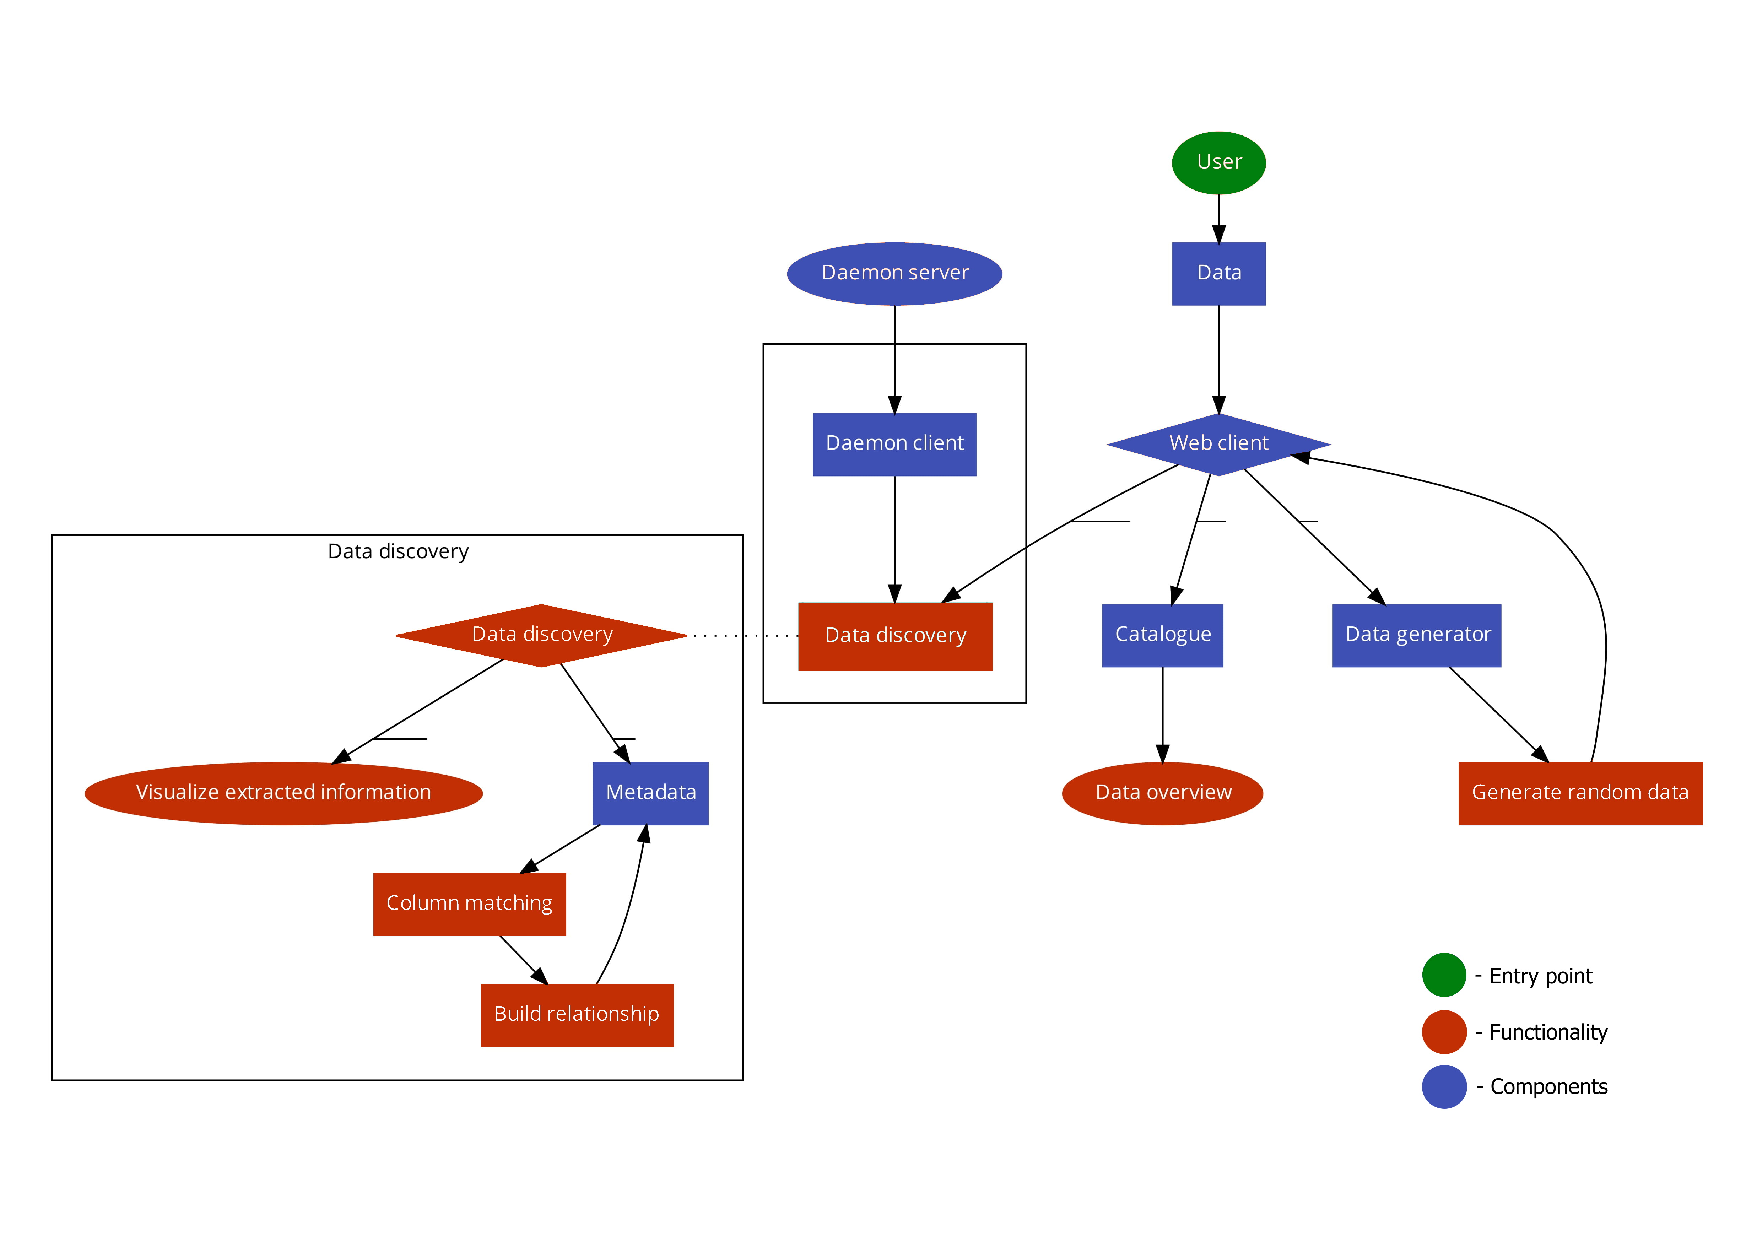
\includegraphics[width=16cm]{figures/architecture}
    \caption {Architecture of the data catalog \& data discovery system}
    \label {fig:architecture_diagram}
\end{figure}

To understand this diagram, we must focus on the core of the system, which consists of two key elements: the metadata and
the data matching library.
We consider these to be of critical importance, because the metadata is our chosen representation of information in the
catalog and the matching library is the primary building tool that gathers and structures this information.
Every other component has merely a supportive role.
We describe the metadata in detail in Section ~\ref{sec:metadata}, and the data matching library in Sections
~\ref{sec:discovery-strategy} and ~\ref{sec:the-data-matching-library}.

We present implementation details in Section ~\ref{sec:discovery-tool-implementation}, as a proof of concept of a system
that can reliably make use of the algorithms included in the library.
We include a web client in Section~\ref{sec:user-interface} that serves as both a management and display tool for the catalog.
For example, the web client is capable of requesting random data to be generated for testing.
Alternatively, for scenarios in which the user might need static reports instead of a full-blown web interface, we implemented
a metadata visualizer (Section~\ref{sec:metadata-visualization}).

The user interface can also be considered a use case of our product.
There are many others we came up with to showcase the various capabilities of our tool, all of them described in
Chapter~\ref{ch:applications}.
In our prototypes, we utilize two kinds of data.
First, there is the real world data.
The advantage of using this kind of data is that we can create a concrete demonstration of the tool's ability to solve problems
encountered by potential users.
The nature of these problems and how our data catalog might come in handy is explained in Section~\ref{sec:real-world-data}.
Then, there is generated data.
While modeled to reflect pattern that might be encountered in a real scenario, this data is clearly artificial (for example,
it can be just a sine wave), but it has the potential to test the performance of our system, by providing us easy access
to large amounts of it, without needing to access expensive sources.
We built our own random data generator, which we showcase in Section~\ref{sec:random-data-generator}.

In order to reach the goal of high system performance, we asked ourselves the question of why or when we would generate or
update metadata.
The answer is, whenever a new file enters the catalog or when an existing file changes.
Therefore, we need a way to check if a file was modified since the last metadata update and a component that can monitor
these changes.
The considerations behind checksum calculation can be found in Section~\ref{sec:checksum-calculation} and the file monitoring
daemon is explained in Section~\ref{sec:daemonized-file-monitoring}.
In testing of this part of the system, we are making heavy use of random data created by our generator.

With this design, we are aiming to achieve and demonstrate a number of key drivers behind a successful data catalog: scalability
(intensive performance testing and monitoring), usability (powerful user interface, variety of realistic use cases), and
innovation (the core of the system unlocks functionality that is not available in the existing solutions on the market).

\vspace{5mm} %5mm vertical space
\subsection{Catalogue}
The catalogue offers an overview of the respective data. Further on, the catalogue will allow the user to see all the column relationship created by the metadata. Additionally, the user can also make changes to his data as for example, hiding unwanted columns.
\vspace{5mm} %5mm vertical space
\subsection{Data generator}
For testing purposes, we decided to create our own random data generator. We ended up with this decision because we believe that this will enable us to mold the data as we would like. Our data generator creates a simple table, and each column can be either numerical or categorical. As the title suggested, the data generated is random and doesn't replicate real life data. In order to combat performance issues, our approach was to abstract each column into its own class in order to build an arbitrary dataframe
on the specified columns. This choice enabled us to generate a big amount of "fake" data that can be easily used to further develop our main tool. An example of this data generator can be found on the web client.
\vspace{5mm} %5mm vertical space
\subsection{Data Discovery}
The goal of data discovery is to analyze and extract insight from the the provided data. The information gathered will be later used by metadata to build potential relationship between the columns in order to provide the user with insightful and relevant information about his data. Further on we can use this information to represent it in a more organized way. Our approach for data discovery was to take two files and try to match columns between those two files using multiple techniques.

\vspace{5mm} %5mm vertical space
\subsection{Metadata}
Metadata is one of the main features of our data discovery tool. The main point of metadata is to use all the information delivered by data discovery in order to create relationship between columns and files. In short, metadata is data that describes data.
\newline
Some of the objectives for our metadata were that we wanted our metadata to generate human-readable information, but at the same time to also use a pre-existing format and have a low overhead. We also didn't want the users to be forced in installing a third party software in order to access the generated databases.
\newline

\clearpage


\section {Existing Results \& Innovation}\label{sec:existing_results_innovation}
\subsection{Existing Solutions on the Market}\label{subsec:existing_solutions_on_the_market}
Initial market research led us to discover many already developed solutions for the implementation of a data catalog.
We will look at three examples of data catalog solutions and outline their key features.
Afterwards, we will present the main selling points of our own solution, explaining how it innovates the already
established data discovery market.

\subsubsection{Alation Data Catalog~\cite{AlationDataCatalog}}
Alation's Data Catalog solution is focused on collaboration and connectivity.
It has five broad, highlighted features:
\begin{itemize}
    \item A wide variety of data sources, such as relational databases, cloud data lakes, and file systems.
    \item ``Seamless'' collaboration and realtime communication.
    \item Natural language search.
    \item The possibility to set rules and enforce policies.
    \item APIs to connect data sources with off-the-shelf BI tools.
\end{itemize}

\subsubsection{IBM Watson Knowledge Catalog~\cite{IBMWatsonKnowledgeCatalog}}
IBM's catalog highlights the benefits of AI-powered data discovery.
Its main feature is its highly extensive search function.
It allows users to search in plain English for tags or contents of their datasets.
It also keeps a history of searches and offers recommendations based on it.
Like the Alation Data Catalog, IBM also permits the creation and enforcement of rules and policies.
Finally, IBM's Data Catalog creates graphs to visualize the data, but that function goes beyond the scope of our project
(recall that our system is meant to provide meaning out of data such that it can be easily manipulated later, using data
visualization tools).

\subsubsection{Google Data Catalog~\cite{GoogleDataCatalog}}
The Google Data Catalog is a service contained within the Dataplex product~\cite{GoogleDataplex}.
Its functionality is rather simple, as it offers the possiblity to catalog data, generate metadata, and manually tag it.
The primary selling point of Google Data Catalog is that it automatically extracts and catalogs data from its other
products, such as BigQuery, Pub/Sub, and Cloud Storage thus leveraging its incredibly popular and vast library of
data solutions.

\bigbreak

This information can help us determine what our project can innovate on the data cataloging scene.
First of all, we need to include some essential features for our solution to be relevant.
Among these, our system should be capable of processing various data formats, as real world sources generally produce
(examples: CSV, JSON, XLS).
Additionally, metadata should be at the forefront of our system's operations.
Going a bit deeper, it appears that none of the existing products presented above focus on building connections between
pieces of data.
Automatic suggestions for how different datasets relate to each other, how similar they are, and whether they might
belong in the same category, or might have the possibility of being merged together, is an incredibly useful feature
for a data discovery system to offer.
For example, a company that deals with sensors, receives dirty data from various sources, and could find it difficult
to put it all together.
A tool with these capabilities could inform the user if two sets of sensor readings are closely related, as they might
be duplicate, or extracted at the same time, etc.
This can extend to tagging.
It is useful to allow the user to set manual tags, but recommending appropriate tags for newly cataloged datasets has
the potential to speed up and simplify the organizational process.
Naturally, tag suggestions would have to rely on already classified datasets (therefore requiring an already established
collection of data), but this feature is still an example of a system becoming more efficient and easy to use over time.
These features will become the highlights of our product and, put together and extended with additional functionality,
can truly bring a fresh option on the market of data catalogs.

\chapter{The Data Discovery Tool}\label{ch:ch2label}


\section{Metadata}\label{sec:metadata}
Having the results available from the Data Discovery tool, only during runtime is severely limiting.
Therefore, the output of the library must be persisted for later analysis.
Moreover, a standardized
metadata format is useful for data representation during runtime for other ad-hoc use cases.
\newline

A practical solution must adhere to several criteria.
Namely:
\begin{enumerate}
    \item It must use a pre-existing format.
    \item Low overhead.
    \item Minimal number of dependencies.
    \item Enforceable data-contract.
    \item Human readable.
\end{enumerate}

The requirement for the pre-existing format is an obvious one.
By using standardized formats such as XML, the need for custom tools to read the generated data would be
eliminated.

The second point is due to performance considerations.
Generating and persisting the metadata must be
with as little disruption as possible, especially considering that IO resources may be limited as the
analysis is running.

The third condition is concerned with portability.
Ideally, the users of the library should not be
forced to install any specialized applications just to read the metadata.
Enforcing this point also reduces the complexity of the Data Discovery tool

Having a data-contract allows the users to trust that the metadata follows certain constraints.
Therefore, the tools dependent on the data discovery library can rely on the metadata, and may generate their own,
to be fed back.

The last requirement, while not the most significant, enables the users to quickly understand the
state of the system, without having to rely on any helper tools.

\subsection{Representation Candidates}

Several options for metadata representation were considered, and each of them was evaluated by the above-detailed criteria.

\begin{enumerate}
    \item SQLite Database.
    \item Centralized metadata file(s).
    \item Individual metadata file for each analysed file.
\end{enumerate}

\textbf{Database approach:}
Initially, a local SQLite database was considered.
This option had many benefits, such as implicitly enforced data-contracts
in the form of the database schema.
Portability was also a benefit, as SQLite databases are encapsulated in a single file.

Performance would have been questionable, because on one hand DBMSes are optimized for multiple concurrent access,
but on the other hand, they inevitably introduce some overhead over simple file operations.

The main reason why this option was ultimately dropped, is that it would force the user to install software that
can access the generated databases.
Also, any other software that may want to consume the data generated will have to have an SQLite driver.

\textbf{Simple, file based approaches:}
Alternatively, the data discovery instance can simply write its results
to the disc, alongside the analysed data.
The output format will ideally follow some established standard such as XML
or JSON.

Of those two, the latter was picked due to its smaller overall footprint.
While XML has some great accompanying standards,
those are not particularly useful for simple data transfer.
The only necessary component is a way to validate the data.

Fortunately JSON schema is a well established option, and is suitable for the project's needs.

The only remaining decision left, was whether to have a centralized file, either on a project or on a folder level,
or to generate individual JSON files for each analysed file.

Having centralized files has the benefit of reduced footprint, and by extension -
better portability.

However, reading and writing into the same file throughout the discovery run is inefficient, and
needlessly complex, purely from a programmer's point of view.

This approach also fails from a readability standpoint, if we consider situations where the user
may only want to look at results from a particular file.

\subsection{Implementation}

Having decided on an approach, the next step was to introduce the metadata generation into the library.
Internally, the proper metadata structure is enforced by classes.

\begin{figure}[H]
    \centering
    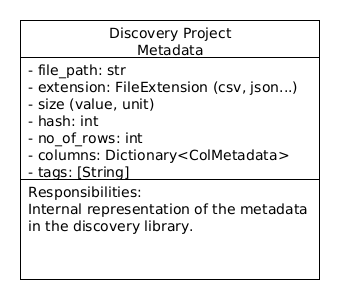
\includegraphics[width=6cm]{figures/metadata/metadata_class}
    \caption{Diagram for the class metadata}
    \label{fig:metadata_fig_1}
\end{figure}



\begin{figure}[H]
    \centering
    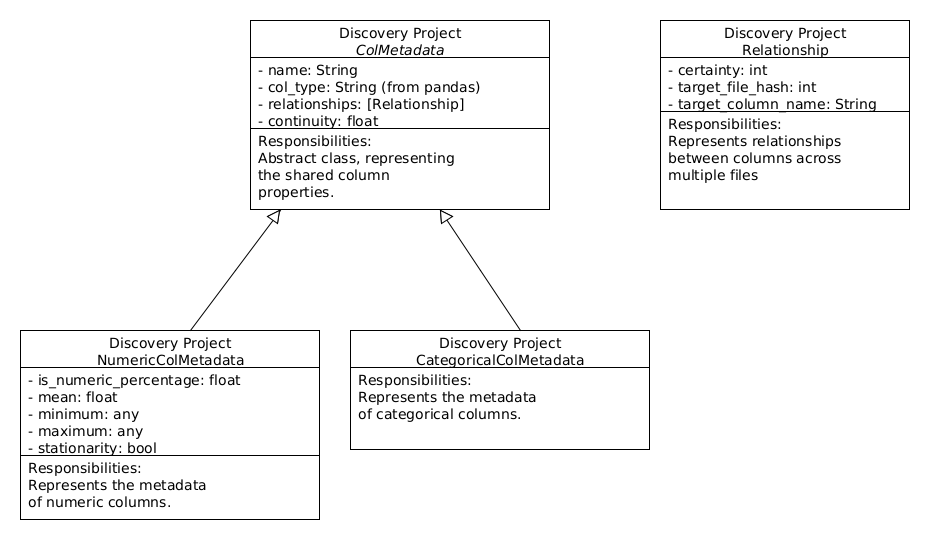
\includegraphics[width=12cm]{figures/metadata/col_rel_class}
    \caption{Diagram for the column and relationship classes}
    \label{fig:metadata_fig_2}
\end{figure}

The exact structure of these classes is as shown on figure ~\ref{fig:metadata_fig_1} and on figure ~\ref{fig:metadata_fig_2}.

After the analysis completes, the results are written into the same folder as the subject file.
The generated file's name has the format of \textit{name-of-the-subject-file.metadata.json}

\newline
\newline

An excerpt from a generated JSON file is as follows:
\begin{lstlisting}[language=json,firstnumber=1]
{
  "file_path": "/mock_filesystem/new_test_0.csv",
  "extension": "csv",
  "size": {
    "quantity": 1336720,
    "unit": "byte"
  },
  "hash": -7102791497049667481,
  "no_of_rows": 5000,
  "tags": [],
  "columns": [
    {
      "name": "Unnamed: 0",
      "is_numeric_percentage": 0.0,
      "continuity": 1.0,
      "mean": null,
      "minimum": "2016-01-01 00:00",
      "maximum": "2016-07-27 07:00",
      "stationarity": 0,
      "relationships": [
        {
          "certainty": 100,
          "target_file_hash": "1464446627197681099",
          "target_column_name": "Unnamed: 0"
        }
      ]
    },
\end{lstlisting}

A notable difference between the generated JSON files and the metadata classes is the
omission of the differentiation between categorical and numerical colum types.

This is due to a late realization, that often values that are not numerical may still have
\("\)numeric like\("\) values such as minimum and maximum. (e.g.\ dates), and those
were implicitly handled by the tools that the implementation relies on.

\subsection{Data-Contract}
As detailed above, it is not enough to just make the metadata available for the users.
Its structure must adhere to a certain set of promises so that its consumers can reliably consume them.

The same principle must also be held up the other way around.
It's easy to reason that in the future third party plugins may be allowed to be part of
the library, in such situation, the library must ensure that the metadata it receives are valid.

Since it's already been established that the project will use JSON as its metadata format,
writing the data-contract in the form of a JSON schema standard ~\cite{jsonschema} was an obvious choice.

It's a simple format, also written in JSON. Moreover, due to its structure, it's human-readable, and self-explanatory.

Below is an excerpt from the JSON schema as implemented (full version is available in the appendix)
\begin{lstlisting}[language=json,firstnumber=1]
{
    "$schema": "http://json-schema.org/draft-04/schema#",
    "type": "object",
    "properties": {
    "file_path": {
      "type": "string"
    },
    "extension": { "enum": ["json", "csv", "parquet"] },
    "size": {
      "type": "object",
      "properties": {
        "quantity": {
          "type": "integer"
        },
        "unit": { "enum": ["byte", "kilobyte", "megabyte", "gigabyte"] }
      },
      "required": [
        "quantity",
        "unit"
      ]
\end{lstlisting}
\ldots
\begin{lstlisting}[language=json,firstnumber=1]
"relationships": {
  "type": "array",
  "items": [
    {
      "type": "object",
      "properties": {
        "certainty": {
          "type": "number",
          "min": 0,
          "max": 100
        },
        "target_file_hash": {
          "type": "string"
        },
        "target_column_name": {
          "type": "string"
        }
      },
      "required": [
        "certainty",
        "target_file_hash",
        "target_column_name"
      ]
    }
  ]
}
\end{lstlisting}

It's worth noting that this schema allows the use of custom JSON fields.
Therefore, it only enforces the inclusion of mandatory fields and the correct form of optional,
but handled fields.

Third party tools are able to add their custom data to the metadata files without making them invalid.
Naturally, in those cases the discovery library doesn't make any promises
about the proper handling of the custom fields.

In the concrete implementation, whenever a metadata file gets read, or written, the
subject string must, first pass through a validation layer before it's allowed to be consumed
or saved.

This behaviour also has the benefit of acting as an implicit test to ensure that library is working
as intended.

\subsection{Generalisation}
Currently metadata exists rigidly to serve locally sourced files.
To distance the solution from this rigidness, some adjustments must be applied for generalisation of what data can be
interpreted as.
Similarly, a generalisation to the data represented in the columns will allow for less rigid explanations of the data
they represent.


\begin{figure}[H]
    \centering
    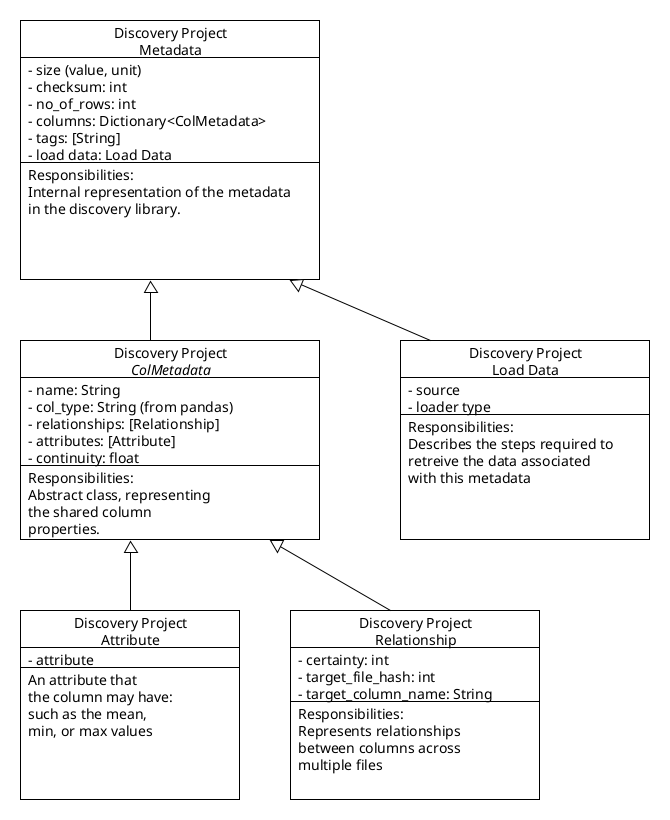
\includegraphics[width=12cm]{figures/metadata/metadata_v2}
    \caption{Diagram for the full metadata layout of a single metadata item}
    \label{fig:metadata_fig_3}
\end{figure}

This new implementation is modeled in fig~\ref{fig:metadata_fig_3} and displays the new abstraction that has been built
that separates metadata from any specific type of existing dataset.
An example of the new proposed structure is as follows:

\begin{lstlisting}[language=json,firstnumber=1,label={lst:lstlisting}]
[
  {
    "ba58f355-c9fa-48b2-aa50-a4afe1343ebb": {
      "data_checksum": 7051072108295319515,
      "no_of_rows": 500,
      "size": {
        "quantity": 28128,
        "unit": "BYTE"
      },
      "tags": {
        "owner": "unknown"
      },
      "loader": {
        "file_path": "matcher_test_0.csv",
        "extension": "csv",
        "data_loader": "LocalCSVReader"
      },
      "columns": {
        "something": {
          "name": "something",
          "attributes": {
            "type": "float64",
            "continuity": 1.0,
            "mean": 52.02349680861937,
            "max": 57.999940436119374,
            "min": 46.00005796296298
          },
          "relationships": [
            {
              "certainty": 10.526315789473683,
              "target_hash": -8333260269495445671,
              "target_column_name": "Unnamed: 0"
            }
          ]
        }
      }
    }
  }
]

\end{lstlisting}

With this implementation, metadata that is required to retrieve data is moved to a new ``loader'' key, as it is now
dependent on the source of the data itself.
Each piece of metadata is also defined by its own UUID, which can be used for indexing when the metadata is saved to any
storage solution.
Furthermore, column attributes have been separated into an ``attributes'' key - this allows the creation of columns that
may have specific data sets with only specific sets of applicable attributes.

In the future this solution allows metadata to describe data that has to be procured in different ways, such as a database
connection, it also allows for big data solutions where the full data set can not feasibly be loaded at a single time.
Lastly, for specialised data, column attributes can be constructed that offer more in-depth descriptions of the column,
such as units for temperature data, or summations in e-commerce data.

\section{Metadata Visualization}\label{sec:metadata-visualization}
During the development of the Data Discovery Library, it was suggested that it would be
nice to have a visual way of communicating the results of the library,
and the general structure of the analysed files.

As a solution, a simple tool was created which can take a list of metadata, and
generated a graphviz file.

\begin{figure}[H]
    \centering
    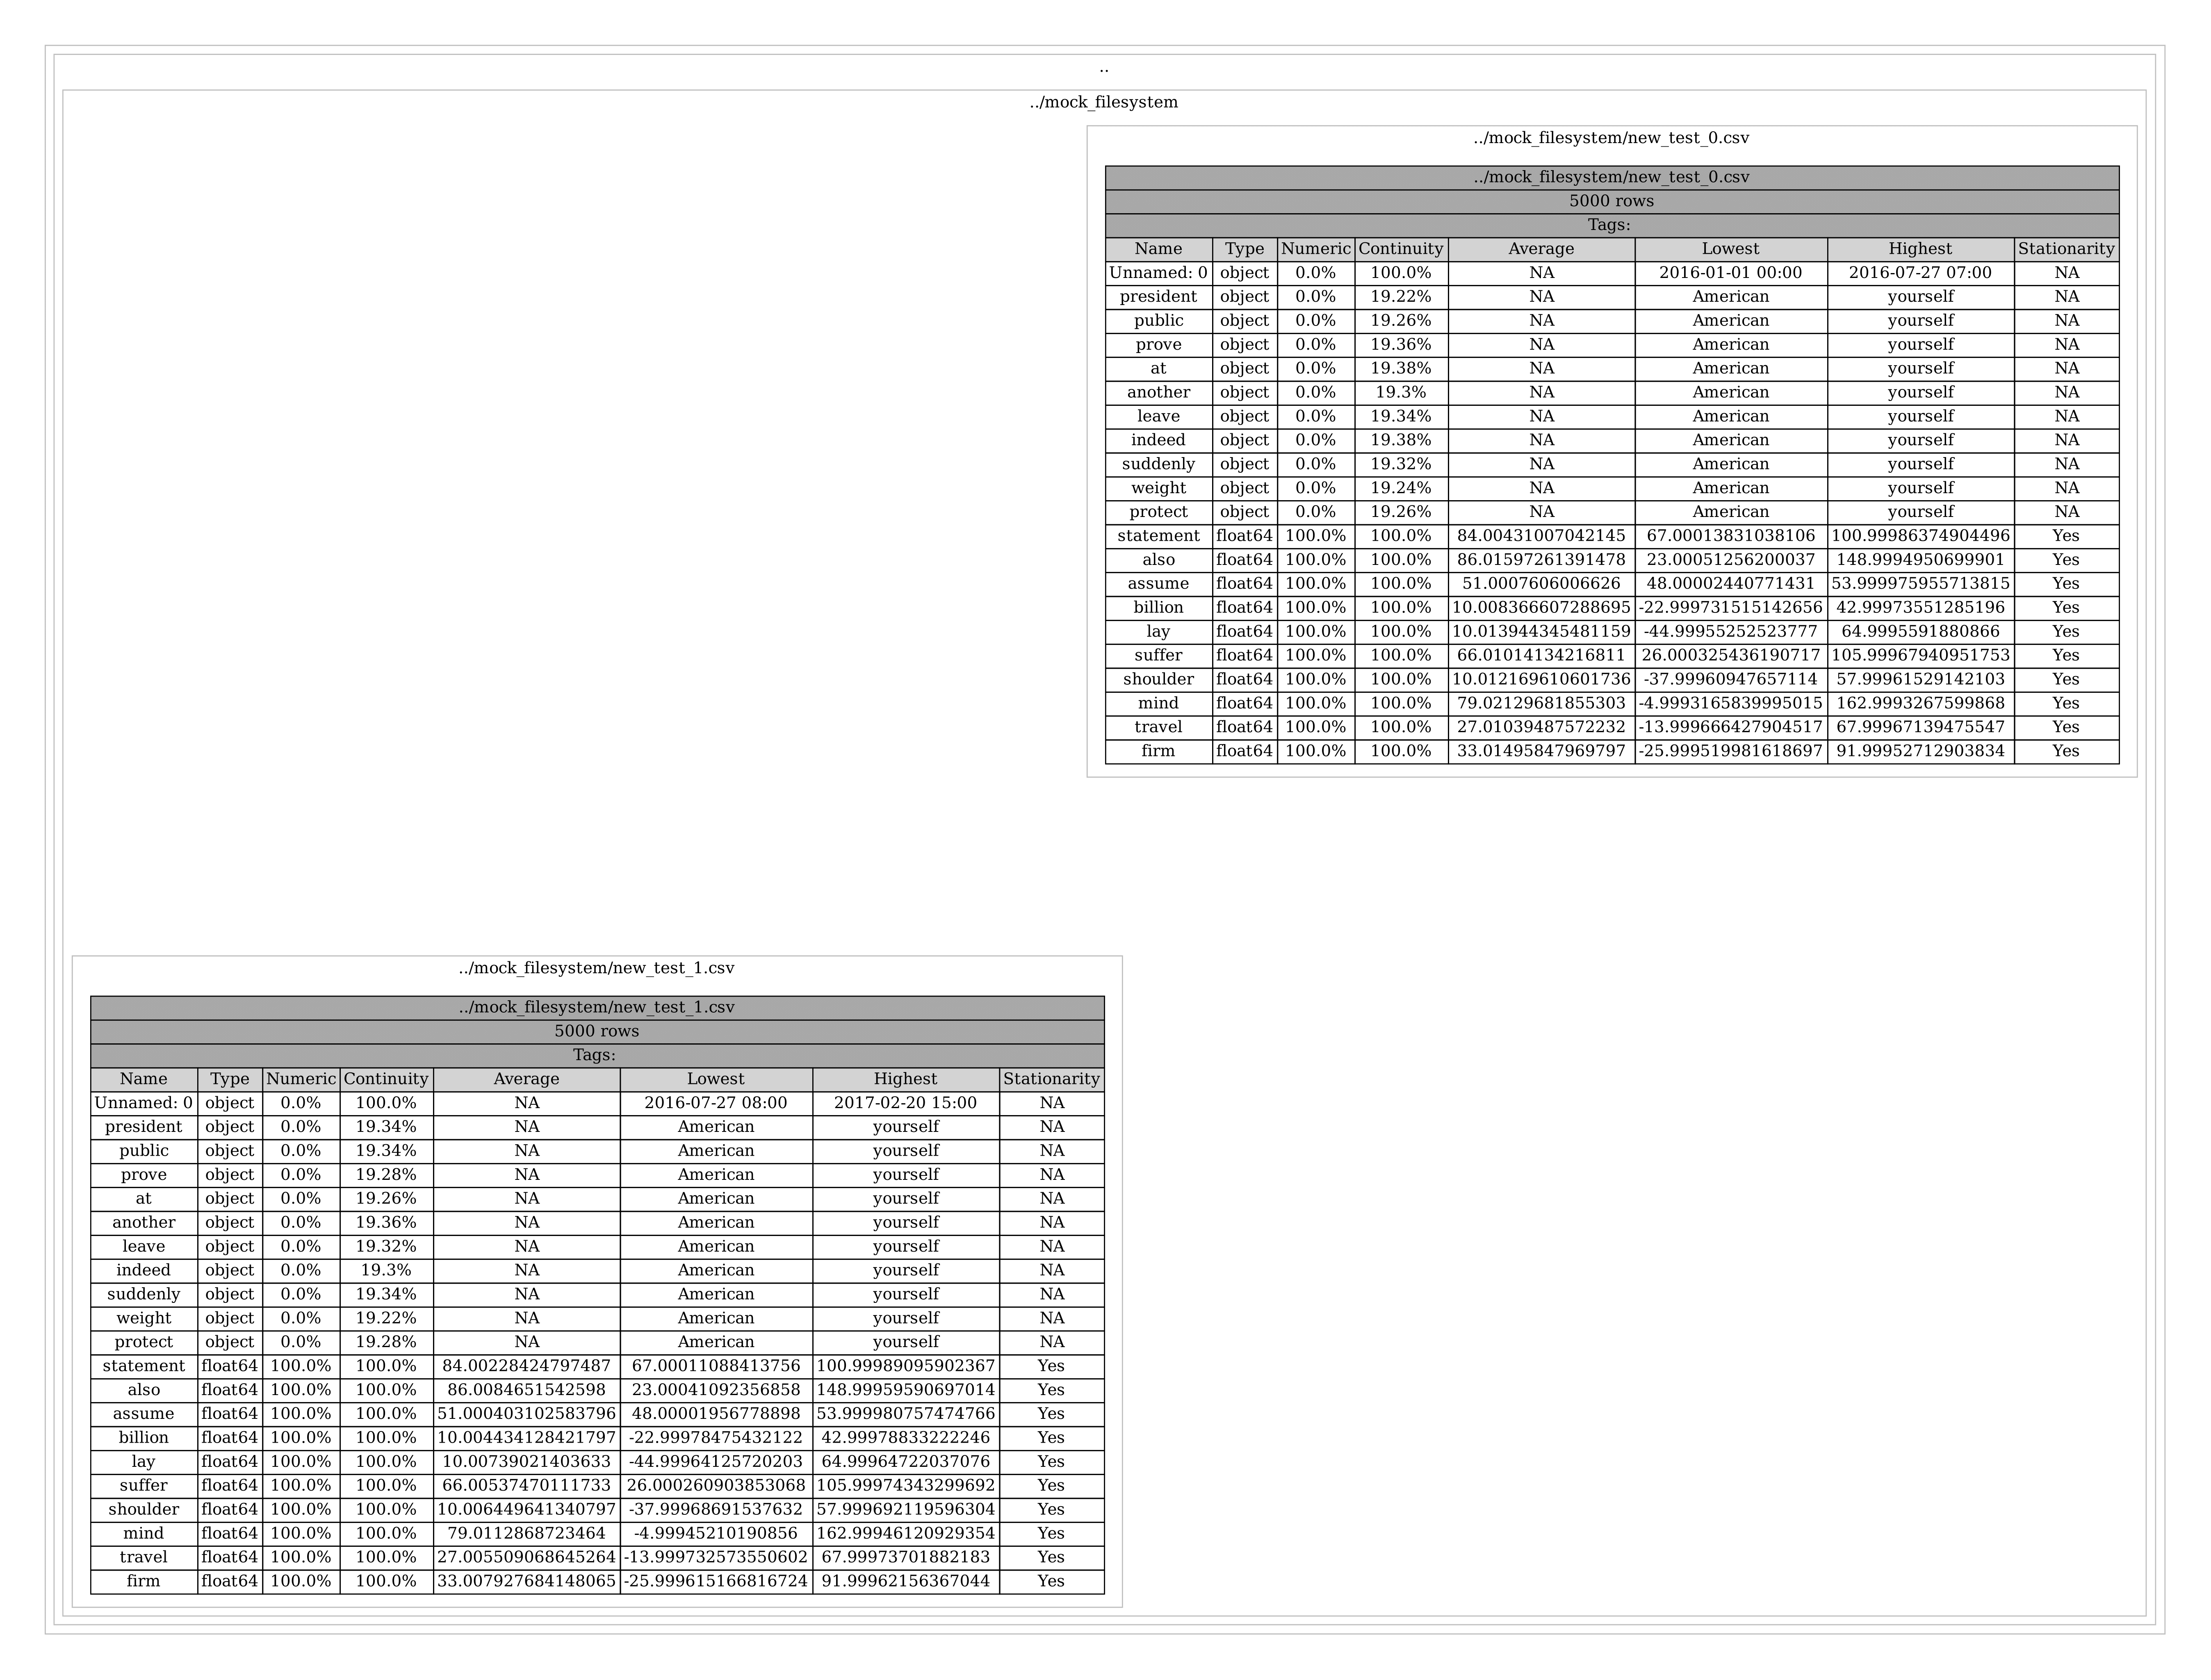
\includegraphics[width=12cm]{figures/metadata_visualization/visualized-1}
    \caption{Rendered output of the metadata visualizer}
    \label{fig:metadata_vis_fig_1}
\end{figure}


An example output is shown on ~\ref{fig:metadata_vis_fig_1}.
Graphviz, as the backing format was chosen because it had a relatively simple,
human-readable syntax - in some cases it even uses HTML tags, for example for tables.
Ultimately, it did become too limiting, when attempts were made
to implement things like relationships across columns.

Internally, to generate the correct structure, the visualizer tries
to build a tree based on the metadata filepaths.

Since the metadata are not guaranteed to be ordered based on depth, the visualizer
iterates through all of them first, ensuring that all possible levels have been addressed
(based on the file paths) and only then renders the graph.





\section{Discovery Strategy}\label{sec:discovery-strategy}
\subsection{Data Exploration}

During the first stages of the project, we implemented prototypes that helped us better understand the goal of the project
and the steps needed to achieve it.
We defined a smaller objective, which would be achieved during the first few weeks of work.
This objective was the construction of a clear map of our data.
In order to gain insights from an unstructured dataset, we first need to extract as much information about it as possible
and represent it in a structured manner.
This is called metadata.
Ralph Kimball describes metadata as ``the DNA of the data warehouse''\cite{Kimball2008} because of its importance in how data is stored.
Exploring the input by extracting and structuring metadata became the first preliminary goal of the project, which we tried
to achieve through prototypes.
\bigbreak
We split this goal further into steps:
\begin{itemize}
    \item Extract basic information about each file (size, number of rows, column names, data types, aggregate functions)
    \item Represent the extracted information in a human-readable manner
    \item Store the metadata in an efficient format
    \item Build potential relationships between files through column matching
    \item Store the results from column matching as metadata
\end{itemize}

\subsection{Column Matching}

Column matching is a naive approach to data discovery.
Just because two columns look similar, it does not mean that the tables are related.
However, it is a good starting point.
Knowing if a table is timestamped and, if it is, which column holds the date \& time information, is incredibly useful for
the larger goal of the project.
In the beginning, we look at two files and try to match columns through various similarity techniques.
The results produced (as, for example, percentages) are then stored together with the rest of the metadata.
In later steps, we can use them to ``label'' columns or tables against an established set of templates.

\bigbreak

We identified three components which can tell whether two columns contain the same kind of data: the column name, the data
type and the content.
The first two are quick to analyse but provide little insight or may even point us in the wrong direction, while the third
element is reliable, but can have a big impact on performance.
Data similarity is an ambiguous topic, but we will nonetheless try to find methods of completing this task, for each of the
three elements of a column.
The results will be expressed as percentages, which we will then average into a final value representing the
\textit{degree of certainty} that two columns contain the same kind of data.

\bigbreak

If we look at column names as strings of characters, we can determine the longest continuous matching subsequence (LCS) between
the two strings, using, for example, Python's \textit{SequenceMatcher} class.
This also provides a method which produces a ratio of similarity, based on the amount of remaining characters after computing the LCS\@.
This approach seems to yield good results when the column names are similar in terms of characters.
An alternative is the Levenshtein distance, which can more accurately show the difference between two sequences.
To improve the quality of results, we can explore another facet of the column names: their meaning.
If we look at these strings as words, we can use a dictionary to check their similarity.

\subsubsection{A comparison between three methods of determining column name similarity}
Word similarity is a vast topic, and it becomes even larger when considering the possibility that column names are not
necessarily words from the dictionary.
We conducted an investigation into the difference between the three methods identified above of exploring this topic,
in order to determine which would be the most beneficial for our project, or whether we should use them together.
Initial tests were run on a hardcoded list of common column names in a commercial or managerial database: customer\_id,
first\_name, last\_name, phone, email, workdept, salary, deptnumb, manager, majproj, etc.

\bigbreak

We ran three algorithms on all pairs of terms in this list:
\begin{itemize}
    \item Longest Continuous (Matching) Subsequence (LCS), as implemented by the Python \textit{difflib} library~\cite{difflib}
    \item The Levenshtein distance, as implemented by the Python \textit{Levenshtein} library~\cite{Levenshtein}
    \item The Wu-Palmer Similarity, as implemented by the Python Natural Language Toolkit (NLTK)~\cite{wordnet}
\end{itemize}

\bigbreak

We developed two different views of the results of these tests, to compare and contrast them.

\begin{figure}[h]
    \centering
    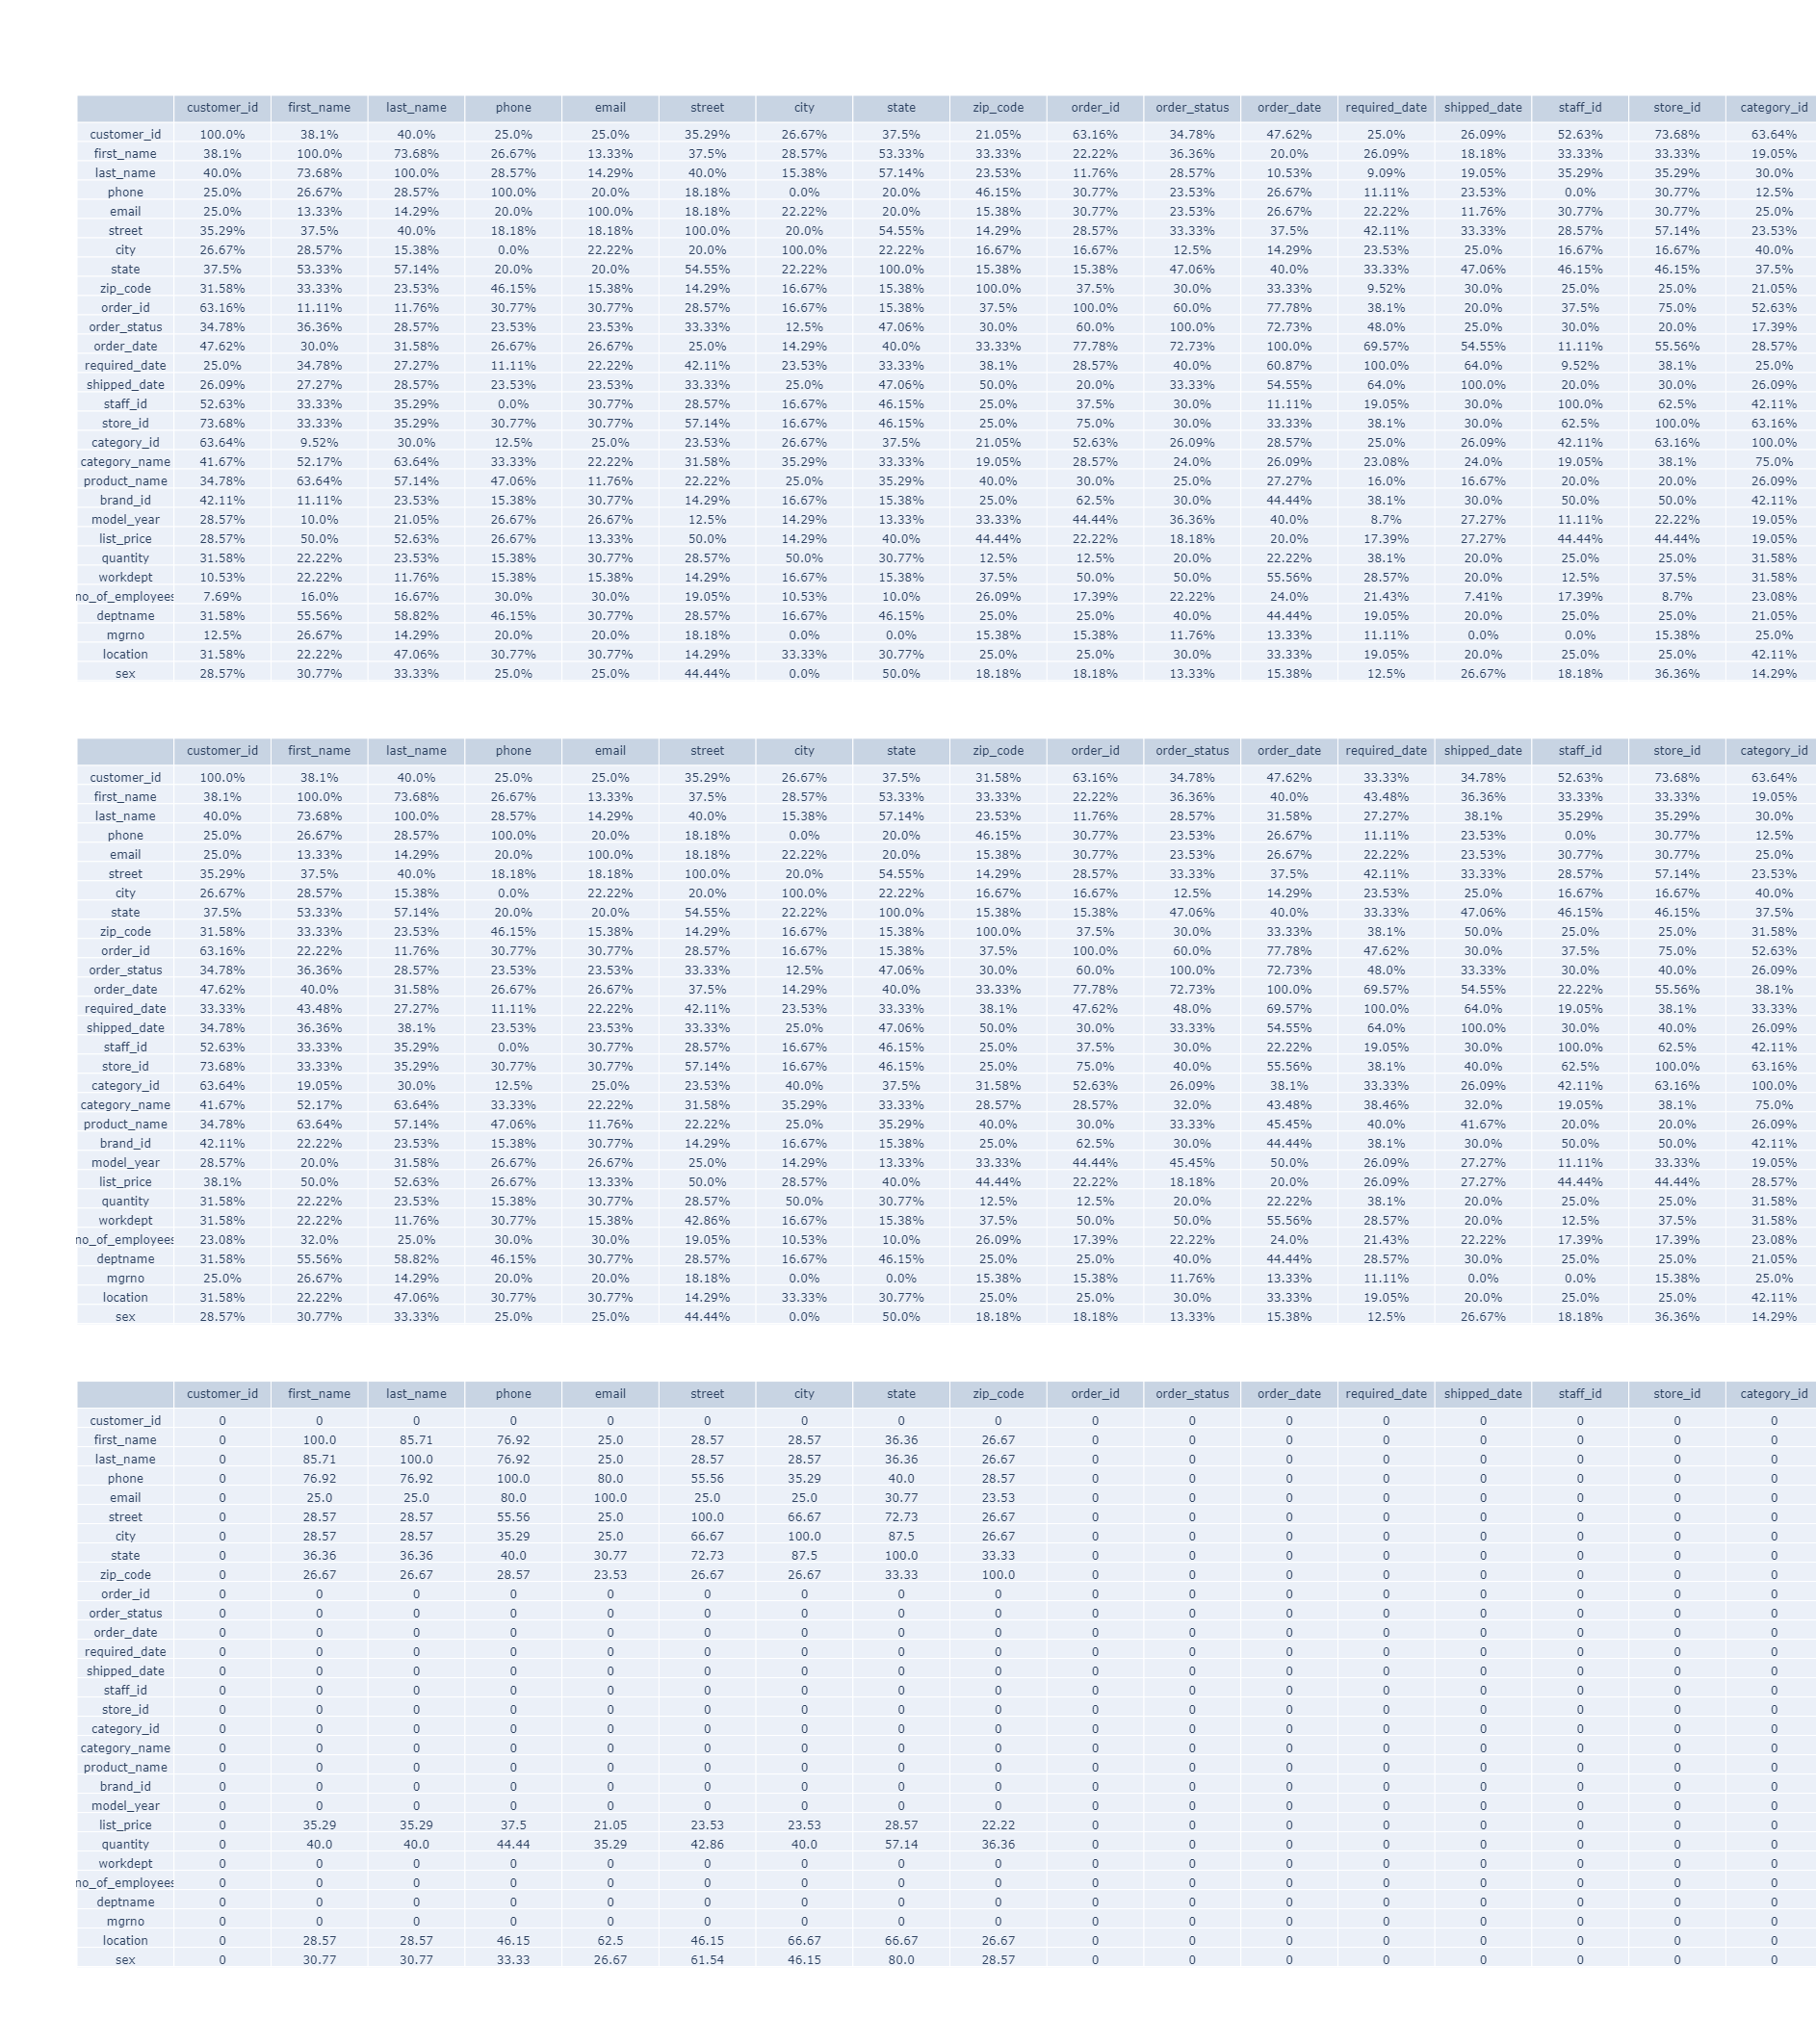
\includegraphics[width=12cm]{figures/names_lcs_levenshtein_wordnet_table}
    \caption{Full results of LCS, Levenshtein, and Wu-Palmer on a list of column names}\label{fig:figure}
\end{figure}

Due to its size, it is difficult to extract any meaningful information from this table.
Nevertheless, at a first glance, we can observe that the values in the LCS and Levenshtein tables are almost identical,
while the Wu-Palmer table contains several zeroes.
To understand these results a bit better, we will a second display method: the best three matches, ranked by percentage,
for each column name.

\begin{verbatim}
hiredate:
	birthdate 70.59%, required_date 66.67%, store_id 37.5% [lcs]
	birthdate 70.59%, required_date 66.67%, firstname 47.06% [levenshtein]
	 0%,  0%,  0% [wordnet]

phone_no:
	phone 76.92%, projno 57.14%, order_id 37.5% [lcs]
	phone 76.92%, projno 57.14%, order_id 37.5% [levenshtein]
	 0%,  0%,  0% [wordnet]

job:
	projno 44.44%, majproj 40.0%, bonus 25.0% [lcs]
	projno 44.44%, majproj 40.0%, bonus 25.0% [levenshtein]
	position 93.33%, zip_code 63.16%, manager 63.16% [wordnet]

position:
	location 62.5%, projno 42.86%, deptname 37.5% [lcs]
	location 62.5%, projno 42.86%, store_id 37.5% [levenshtein]
	location 100.0%, job 93.33%, quantity 61.54% [wordnet]

firstname:
	first_name 94.74%, lastname 70.59%, deptname 58.82% [lcs]
	first_name 94.74%, lastname 70.59%, deptname 58.82% [levenshtein]
	 0%,  0%,  0% [wordnet]

lastname:
	last_name 94.12%, firstname 70.59%, category_name 57.14% [lcs]
	last_name 94.12%, firstname 70.59%, category_name 57.14% [levenshtein]
	 0%,  0%,  0% [wordnet]
\end{verbatim}

This is a fragment of the results displayed as the best three matches for each column name.
Every row represents the results of one method used.
Once again, we observe that LCS and Levenshtein results are very similar.
In cases where they do differ, they seem to both miss the mark.
For example, LCS matches \textit{hiredate} with \textit{store\_id} with a 37.5\% confidence, while Levenshtein matches
\textit{hiredate} with \textit{firstname} with a 47.06\% confidence.
Both pairs of column are most likely unrelated.
However, when it comes to column names with slight variations in spelling, such as \textit{lastname} and \textit{last\_name},
both LCS and Levenshtein produce correct matches with a 90\% or higher confidence.
Wu-Palmer (wordnet) fails to match columns that are not correctly spelled words in the dictionary.
On the other hand, Wu-Palmer can find matches that are essentially invisible to LCS and Levenshtein.
For example, it matches \textit{position} with \textit{location} with a 100\% confidence, which is correct (both of these
columns might contain physical locations), but it also matches \textit{position} with \textit{job} with a 93.33\% confidence,
which is also a valid option (position might refer to an employee's function in a company).

\subsubsection{Understanding the results}
According to the Python documentation, the algorithm behind SequenceMatcher predates an algorithm published by Ratcliff
and Obersheldp in the late 1980's under the hyperbolic name ``gestalt pattern matching''~\cite{difflib}.
The idea is to find the longest contiguous matching subsequence, and then apply it recursively to the sequences to the
left and right of the matching subsequence~\cite{difflib}.
The \textit{ratio()} method return a float in the range [0, 1] with the formula 2.0 * M / T, where T is the total number
of elements in both sequences and M is the number of matches~\cite{difflib}.
The Levenshtein distance between two strings is the number of insertions, deletions, or substitutions required to transform
one string into the other.
A C extension module for Python implements the ratio of similarity between two strings as the complement of the normalized
Levenshtein distance~\cite{Levenshtein}.
Given these implementations of LCS and Levenshtein, it makes sense that the results obtained are very similar.
Both methods look at how close two strings are character by character.
Therefore, the best usage of these methods in column name matching is to combine them.
Disagreements with a low confidence percentage can be ignored, but disagreements with a high confidence should be resolved
by applying a different comparison method, such as Wu-Palmer.

\bigbreak

WordNet is an interface for Python's NLTK module.
According to its documentation, WordNet structures words using synsets, which are, essentially, sets of synonyms that
share a common meaning~\cite{wordnet}.
Each synset contains one or more lemmas, which represent a specific sense of a specific word~\cite{wordnet}.
The Wu-Palmer similarity is implemented as ``a score denoting how similar two word senses are, based on the depth of the
two senses in the taxonomy and that of their Least Common Subsumer (most specific ancestor node)''~\cite{wordnet}.
This explains why our Wu-Palmer test was able to match \textit{position} and \textit{location}, but also \textit{position}
and \textit{job}, both with a very high confidence.
The word ``position'' shares a synset with both ``location'' and ``job'', the first one meaning ``a place in the physical world'',
and the second one ``a function in an organization''.
This algorithm is, therefore, extremely useful for identifying columns with similar data, whose names are synonyms in the
dictionary.
The shortcomings of WordNet are visible when the words are spelled incorrectly.
For example, the algorithm might correctly identify the words \textit{first} and \textit{name}, but not \textit{firstname},
nor \textit{first\_name}, the last two being common occurrences in datasets.
A possible solution is the use of tokenization (splitting a string into words).
However, attempts to use this approach did not show an improvement of results.
That is because many of the common column names selected in the test (such as \textit{firstname} and \textit{majproj}) cannot
be tokenized.
Additionally, WordNet does not work well with phrases.
Its synsets are built with singular words, therefore it cannot grasp the meaning obtained when combining words such as
\textit{phone} and \textit{number}.

\subsubsection{Data types}
The data types provide the least amount of information about the similarity of the two columns.
We can check whether they share the same data type (numerical, strings, boolean), but this does not mean the contents
are related.
However, finding numerical data gives a strong probability that the data in the column is continuous, while finding any other
data type may show that the data is categorical.
\todo{Add reference}
Unfortunately, this can only be verified by looking at the data itself.
Looping through the rows and comparing them is costly.
If we are dealing with categorical data, there might be value in comparing the sets of categories and their frequencies.
\todo{Show results}
Continuous, numerical data can be compared using mathematical formulas, such as the Pearson correlation coefficient.
\todo{Add reference}
\todo{Show results}

\subsubsection{Stationarity}
A stationary process is ``a stochastic process whose unconditional joint probability distribution does not change when shifted
in time''~\cite{Gagniuc2017}.
In other words, it is ``a flat looking series, without trend, constant variance over time, a constant autocorrelation structure
over time and no periodic fluctuations''~\cite{EngineeringStatisticsHandbook}.
Determining whether our continuous data is stationary or not could be the first step towards trend analysis and prediction.
Stationarity can by itself be an indication of similarity (for example, temperature measurements taken at the same place
in the same season should be stationary), but it should be combined with other kinds of analysis for higher accuracy.
One method of determining stationarity is the Augmented Dickey-Fuller Test (ADF).
ADF tests the null hypothesis that a unit root is present in a time-series sample~\cite{Greene1997}.
If a unit root is present in a stochastic process, then that process is non-stationary, but it does not necessarily have a trend.
Therefore, the alternate hypothesis of the ADF test is that the series is stationary.
ADF uses the p-value to accept or reject the null hypothesis, but it also produces a secondary value, called the ADF statistic.
The more negative this number is, the stronger the confidence in rejecting the null hypothesis~\cite{Greene1997}.

\bigbreak

The Python library \textit{statsmodels} contains an implementation of ADF~\cite{statsmodels}, which we applied to data produced
by our generator.
Our test dataframes are composed of two columns and one hundred rows.
The first column is an index, and will always have values from 0 to 99.
Running ADF on this series produces an ADF statistic of approximately 2.46 and a p-value of 0.99.
This is extremely strong evidence for accepting the null hypothesis that this series is non-stationary, which must be true
for a linear, incremental process.
The second column will always contain continuous data following a sine wave.
All tests on this column produced small ADF statistic values, around -5000000000000.
The p-value was shown as 0.0, indicating that it was a positive number very close to 0.
This evidence points towards confidently rejecting the null-hypothesis that the series has a root value and claiming that
a sine wave is stationary, which, once again, is true.

\bigbreak

Given the varying significance of these results, adding weights to the final computation is crucial.
\todo{How?}



\section{The Data Matching Library}\label{sec:the-data-matching-library}
The algorithms from the previous section were compiled into a library for data matching and exploration.
There are several reasons for this design choice, which become obvious when we look at the alternative.
Another possibility would have been to create services that process one or more dataframes with all the available methods
and return the result.
However, a library is much more flexible.

First of all, by storing methods in a library and calling them from the matcher service, we offer the user the option to
only select the relevant methods for the task at hand.
This is important because, while we can determine when a method is technically inapplicable (for example, two-sample T-test
only works on continuous, numerical series), there are many ambiguous scenarios where trying out different combinations of
methods on the same dataframes can provide noteworthy results.

Second of all, it is a question of performance.
The following is one layer of the structure of our data matching library, showcasing different types of methods based on
how they interact with the data.

\begin{figure}[h]
    \centering
    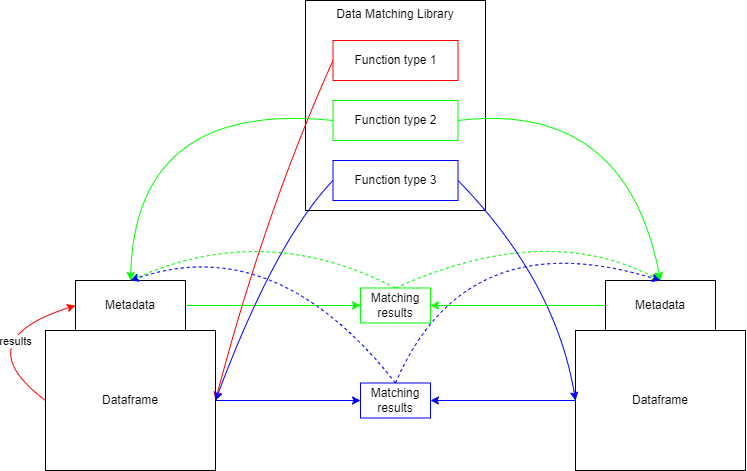
\includegraphics[width=12cm]{figures/data_matching_library/data_matching_library}
    \caption{Data matching library method types}
    \label{fig:data_mathicng_library_doc_1}
\end{figure}

This is just one possible classification, but it is useful for identifying performance differences and deciding how to
handle results.
The first method type (red) is applied on the dataframe and generates results which should be included in the metadata.
These are metadata builder methods such as the Augmented Dickey-Fuller Test for stationarity, the formula for calculating
the percentage of numerical values in a column, and the formula for calculating the continuity factor of a column.
These results are expensive to calculate and, therefore, should be included in the metadata, as they will be used in further
exploration and matching algorithms.

The second method type (green) uses the metadata of two dataframes to generate similarity or correlation estimates.
These methods help create a network of data structures and reveal information about seemingly unrelated pieces of data.
They are computationally efficient, because they only use metadata, without accessing the dataframe rows, so, at least
in theory, we could compute these results as often as we need them.
However, it is still useful to store some of them in the metadata, for example, similarity percentages between the columns
of two particularly related dataframes, as they may be displayed to the user in different formats or sent for further processing.
Examples of methods of type two include all name matching methods, comparisons of column aggregates (such as minimum, maximum,
and mean values), and comparisons of the results of type one methods (continuity, numerical percentage and stationarity).

Finally, the third method type (blue) uses the actual rows of a dataframe to generate similarity estimates.
These results are expensive to compute, and therefore should be stored in the metadata and reused from there instead of
calculated from scratch whenever possible.
Methods of type three include matching identical rows, calculating the Pearson coefficient, performing the two-sample t-test,
and the Dynamic Time Warping algorithm.

The question that remains is how to store matching results in the metadata.
Do we store them in the metadata files attached to both dataframes or only in one of them?
And do we store every result for every single column?
The answer is: it depends.
If we are exploring the data from the perspective of one test dataframe, which we want to know more about, then it is
sufficient to store matching results only in its metadata file.
For example, we might want to store the top N most similar columns to each column in our dataframe, after exploring the entire
data catalog.
However, there are situations in which we must store results in both metadata files of dataframes under comparison, because
the obtained percentages might not be mutual.
For example, when determining the best column match in dataframe B for every column in dataframe A, the results may differ
if we swap the dataframes around.
We must also pay attention to how fast the obtainable information in our data catalog grows.
Storing every similarity percentage between any two columns in any two dataframes is not feasible in the long run, as the
space complexity of such an endeavor is quadratic on the total number of columns in the data catalog.
The solution is to identify dataframes of interest where we temporarily extend the metadata with column relationships.
Use cases where we exemplify these techniques will be present in the following chapter.

One final component that we need in order to utilize this library is an interface that can receive all relevant parameters
and run one of the matching methods in the library.
The list of parameters must include the name of the method that should be called, the metadata information of the two columns
that we are trying to match (if the method performs computation on two columns), the columns themselves (if the method needs
to access the data rows), and the metadata information of the two dataframes to which the columns belong.
The last parameter is relevant because storing a column relationship in a metadata file requires some kind of identifier for
the second column beyond its name.
For this, we can use the hash of the file containing its dataframe.
The concept of hashing large files and the various performance considerations behind it will be discussed in a different chapter.



\section{Checksum Calculation}\label{sec:checksum-calculation}
In order to uniquely identify the files analyzed, and detect changes across runs, the Data Discovery Library must
perform some calculations on each file to generate a unique ID that is dependent on the content of the file.
Ideally these calculations are efficient and the generated IDs will have a low collision rate.

\subsection{Hashing, CRC and Checksum Algorithms}
Before deciding on the algorithm that will be used to generate the IDs, it's important to clear up the differences
between hashing, checksum and CRC algorithms.
These terms are often used interchangeably (e.g.\ the metadata generated by the library also uses the term \("\)hash\("\)
as a place-holder for the ID field)

Arguably, these operations achieve similar results, i.e.\ taking an unknown sized chunk of data, and reducing it into
a constant n-sized output value.
However, they are intended for different use cases.
The goal of a hashing algorithm is to create values that have low
collision rates, they are also often used for cryptographic applications (which is irrelevant for this project).
The low collision rates however comes at the cost of slower computation rates, compared to checksum algorithms.
The values generated by hashing algorithms are referred to as digests.

\newline

Checksum and Cyclic Redundancy Check Algorithms both aim to detect errors in the files.
Of course, by extension this
also means that files with minor changes are guaranteed to have different checksum values.
They usually have
faster computation rates compared to hashing algorithms due to their smaller sizes and lack of cryptographic concerns.
Naturally, the smaller checksum sizes do increase the chances of collisions.

The difference between CRC and checksum algorithms is the method of calculation.
CRCs are slower, but able to generate larger error runs.

\subsection{Collisions and the Birthday Problem}

Since the generated values, are meant to be used as unique identifier for files and to track changes of the files, it's important
to discuss collision rates. Figure ~\ref{fig:checksum_fig_1} shows the birthday problem in action.
Essentially, if there are 77163 files, by using a 32-bit checksum, the odds of a collision is 50\%.

Therefore, there must be a careful balance between performance and coliision rates.

\begin{figure}[H]
    \centering
    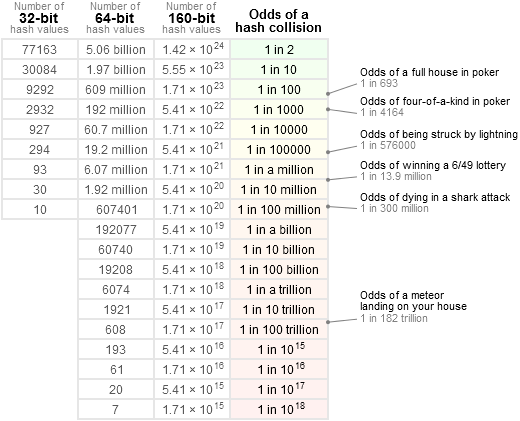
\includegraphics[width=12cm]{figures/checksum/collisions}
    \caption{Chances of collision for various bit sizes, source: ~\cite{PreshingCollisions}}
    \label{fig:checksum_fig_1}
\end{figure}



\subsection{Offloading the Hash Calculations into Compiled Modules}
Before investigating the various CRC and checksum algorithms.
It is beneficial to consider offloading the checksum calculations into a separate, compiled module.
It is easy to do so, since:

\begin{itemize}
    \item There isn't much interdependency between the checksum calculation and the rest of the library.
    \item The generated values are numeric, which are unlikely to cause conversion issues across the modules.
    \item Python has a well established culture, of offloading calculation heavy processes into compiled modules.
\end{itemize}

To test this idea, Rust was chosen as it enables its users to write low level code, while still being memory safe.
Its performance is also comparable to C. That being said, the results here are reproducible on any compiled, low level
language, assuming it can interface with Python.

The modules were always compiled with the release flag on.
The python wheels were generated using Maturin ~\cite{Maturin}.

\begin{table}[]
\begin{tabular}{ll}
Operating System  & Ubuntu 22.04.1 LTS x86\_64                                     \\
Kernel Version    & 5.15.0-56                                                      \\
Processor         & Intel i7-4700MQ @ 3.400GHz                                     \\
Memory            & 16Gb DDR3 @ 1867MHz                                             \\
Hard drive        & SATA SSD @ 452.62 MB/s read                                    \\
Aggregate Size    & 100GB                                                           \\
File Distribution & 10000 uniformly sized 10mb files containing output from urandom
\end{tabular}
\caption{Benchmark Environment}
\label{tab:checksum_tab_1}
\end{table}

The specifications of the benchmark environment are as shown on ~\ref{tab:checksum_tab_1}.
Initially, to validate the assumption that offloading the checksum calculation will cause a reduction
in runtime, a simple test was created.

The test compares the single threaded performance of Python and Rust calculating CRC32 checksums.
Each of them iterate over a list of file paths, following these steps:
\begin{enumerate}
    \item Open file at offset (starting at 0).
    \item Create empty CRC32 generator.
    \item Read the contents into a 131.072 KB buffer (1024 * 128 bytes).
    \item If EOF, push the generated checksum into a list of results (go to step 1).
    \item otherwise update the generator with the content of the buffer.
    \item Increase the offset.
    \item Go to step 3.
\end{enumerate}

\begin{figure}[H]
    \centering
    \begin{bchart}[step=50,max=350, unit=s]
        \bcbar[label=Python]{326}
        \medskip
        \bcbar [label=Rust]{307}
    \end{bchart}
    \caption{CRC32 single threaded calculation speed (lower is better)}
    \label{fig:checksum_fig_2}
\end{figure}


The results (shown on figure ~\ref{fig:checksum_fig_2}) indicate,
that while the speed increase is not significant,
there is a consistently reproducible speed increase when the CRC calculations are done with Rust.


\subsection{Comparison of various Checksum and CRC Algorithms}

Having established that compiled solutions are the way forward, it was still important to compare various CRC and checksum algorithms.
The main focus was on performance, as the various collision rates were already established.

This project investigated three different algorithms (although there are many available).
Namely:
CRC32, Adler32 and Fletcher16.

\begin{figure}[H]
    \centering
    \begin{bchart}[step=50,max=400, unit=s]
        \bcbar[label=CRC32]{307}
        \medskip
        \bcbar [label=Adler32]{310}
        \medskip
        \bcbar [label=Fletcher16]{313}
    \end{bchart}
    \caption{Comparison of various algorithms (lower is better)}
    \label{fig:checksum_fig_3}
\end{figure}

As shown on ~\ref{fig:checksum_fig_3}, the algorithms performed similarly to each other.
This is odd, in the sense that previous research ~\cite{MaxinoChecksum} found that Adler32 outperforms CRC32,
and Fletcher16 outperforms the former.

A possible explanation why these results were not reproduced here, is that this project uses off the shelf
solutions for calculating the checksums.
Therefore, the level of optimization will vary between the used packages.
Creating new implementations for these algorithms is outside the scope of this project.
While in theory, it should be possible to create a better optimized version of Adler32, it is easier
to use the CRC32 package, as it is faster, and has all the other benefits of using CRC32 over Adler32.

\subsection{Introducing Parallelism}
All the previous implementations (excluding the checksum calculators, of which there are no assumptions made),
ran sequentially.
It is, however, simple to introduce parallelism.
One may create a threadpool, from which threads can receive jobs (file paths) from a source list.
The worker thread then sequentially calculates the checksum for the file, and then returns the result.

This way the number of race conditions are limited.
First, the distribution of the jobs from a single source list.
This is a common pattern, and there are many readily available solutions.
In this specific instance, Rayon  ~\cite{Rayon} - a popular data-parallelism package was used.

\begin{figure}[H]
    \centering
    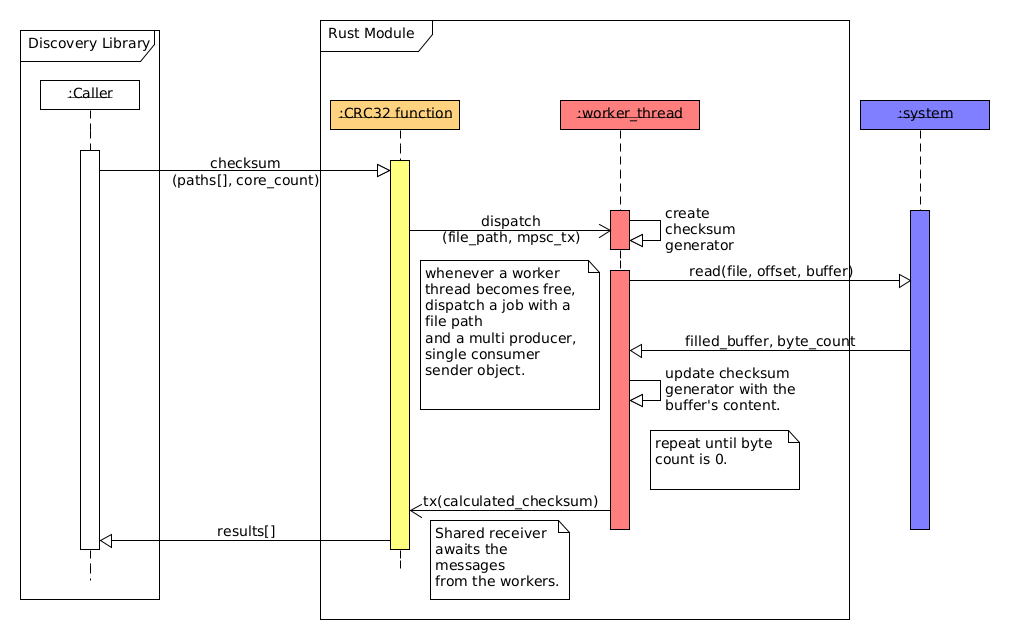
\includegraphics[width=12cm]{figures/checksum/simple_multi_crc}
    \caption{Sequence diagram for a parallelized checksum function.}
    \label{fig:checksum_fig_4}
\end{figure}

The second opportunity for race conditions is when the results are collected.

Figure ~\ref{fig:checksum_fig_4} shows the general flow of the parallelized CRC32 function.
The communication
between the main thread and the worker threads was implemented by using an MPSC FIFO queue (Multi-producer, single-consumer)
each thread receives a sender object, which is used to push their results into the queue.
Finally, after each job finished, the main thread, using the receiver object collects and returns the results to the caller.

The order, in which the results are collected is irrelevant, as it is easy to extend the above flow to include
the file path alongside the calculated checksum (it was omitted, as these tests are purely for benchmarking purposes).
Therefore, the potential for a race condition when collecting the results is also resolved.

\begin{figure}[H]
    \centering
    \begin{bchart}[step=50,max=400, unit=s]
        \bcbar [label=Original, no paralellization]{307}
        \medskip
        \bcbar[label=2 threads]{210}
        \medskip
        \bcbar[label=4 threads]{201}
        \medskip
        \bcbar[label=8 threads]{203}
        \medskip
        \bcbar[label=16 threads]{209}
        \medskip
    \end{bchart}
    \caption{Performance comparison for various thread counts when running the parallelized CRC32 function.}
    \label{fig:checksum_fig_5}
\end{figure}


The introduction of parallelism, did result in significant performance gains ~\ref{fig:checksum_fig_5}.
It is interesting to note, that when the thread count was above four, the performance started to decrease again.
A possible explanation for this is that the test computer has a four core processor, so it is possible that number of context
switching significantly increases after the thread count exceeds the core count (although this explanation
ignores hyper-threading).

\subsection{The IO Problem}
Calculating checksums is a relatively efficient process, to the point that
some processor instruction sets even include CRC32
as a built-in instruction~\cite{CRC32Instruction}.

The main bottlenecks therefore, are the IO operations.
This bottleneck becomes apparent when multiple checksums are calculated in parallel.
This is especially true when the files are stored on a hard-drive ~\cite{PiotrParallelDiskAccess}.

Essentially, the threads are competing for the same resource (disk access), slowing each other down.

\begin{figure}[H]
    \centering
    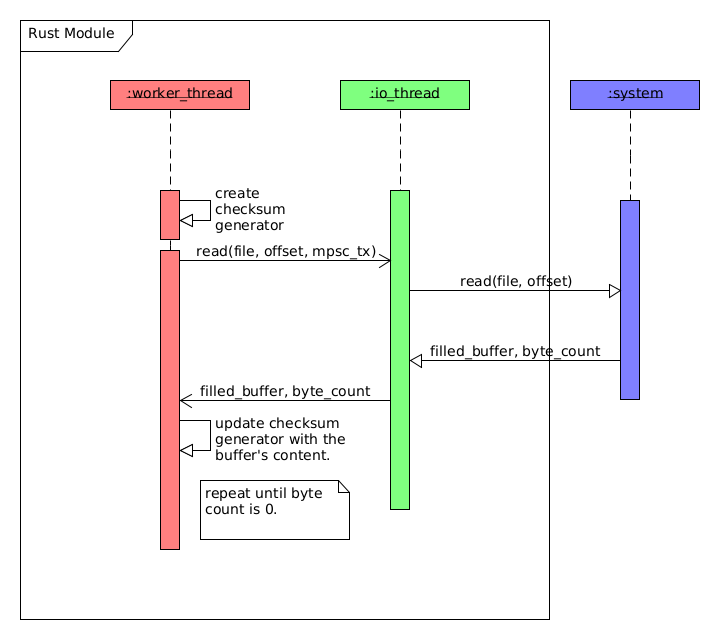
\includegraphics[width=12cm]{figures/checksum/io_multi_crc}
    \caption{Multithreaded CRC32 function, with dedicated IO thread.}
    \label{fig:checksum_fig_6}
\end{figure}

A common solution is to introduce a dedicated IO thread (shown on ~\ref{fig:checksum_fig_6}), from which, each worker thread could
receive the next piece of data to process.

\begin{figure}[H]
    \centering
    \begin{bchart}[step=50,max=400, unit=s]
        \bcbar[label=2 threads]{375}
        \medskip
        \bcbar[label=4 threads]{352}
        \medskip
        \bcbar[label=8 threads]{351}
        \medskip
        \bcbar[label=16 threads]{348}
        \medskip
    \end{bchart}
    \caption{Parallelized CRC32 calculations with dedicated IO thread}
    \label{fig:checksum_fig_7}
\end{figure}


This approach, as it is apparent from the results on ~\ref{fig:checksum_fig_7} caused considerable slow downs,
even compared to single threaded performance.

This slow down, first, can be attributed to increased context switching.
Second, it was also implemented using MPSC queues.
While these queues are great to send simple values back and forth, they were inefficient
when they were used to pass along large buffers, as each time the buffer was sent to the queue,
it had to be copied from the original memory location.

A solution to the latter would be to reimplement the inter-thread communication with shared memory buffers.


\subsection{Solving the IO problem with io\_uring}
Instead of reimplementing ~\ref{fig:checksum_fig_6} with shared memory buffers, an alternative
solution was implemented.

Io\_uring ~\cite{IO_uring} is a novel way of performing asynchronous IO on Linux.
It also claims to increase the performance of multithreaded IO processes.

It relies on two queues, a submission queue (SQ) and a completion queue.
The client simply passes a submission queue entry (SQE), containing the buffer to be filled,
the target file and the offset.

This submission system call is non-blocking, therefore the client may perform other operations
while the system completes the request.
When the client is ready to consume the results,
it can access them from the CQ\@.

\begin{figure}[H]
    \centering
    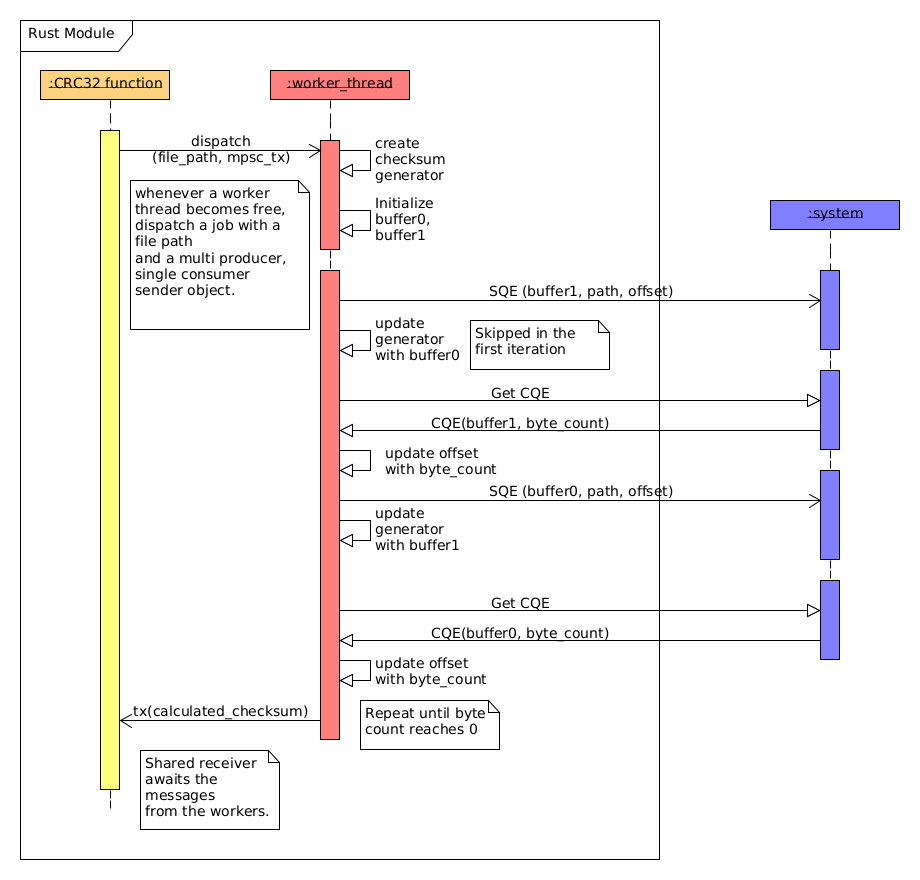
\includegraphics[width=12cm]{figures/checksum/uring_multi_crc}
    \caption{Implementation of the CRC32 function using io\_uring.}
    \label{fig:checksum_fig_8}
\end{figure}

The great benefit of async IO is (as shown on ~\ref{fig:checksum_fig_8}) is that worker threads
don't have to stay idle until the read operation completes.

This behaviour was achieved using a pair of buffers, where one buffer gets processed, while
the other gets refilled.

\begin{figure}[H]
    \centering
    \begin{bchart}[step=50,max=400, unit=s]
        \bcbar[label=2 threads]{213}
        \medskip
        \bcbar[label=4 threads]{197}
        \medskip
        \bcbar[label=8 threads]{202}
        \medskip
        \bcbar[label=16 threads]{206}
        \medskip
    \end{bchart}
    \caption{Parallelized CRC32 calculations using io\_uring.}
    \label{fig:checksum_fig_9}
\end{figure}

Some, minor improvements were achieved (~\ref{fig:checksum_fig_9}), but its results were comparable
to the simple, parallelized approach.
This may be attributed to the implementational overhead of using io\_uring.
Alternatively, it is possible that it wasn't designed to be used in such a way, and with
a different approach it could provide greater improvements.

Finally, these benchmarks were executed on an SSD, which perform better when accessed in parallel.
It is probable that, when ran on mechanical hard disk, the usage of io\_uring would achieve
greater differences compared to the original parallel approach.

\subsection{Conclusion}
First, these solutions are not fully optimized.
There are countless ways to shave off a few seconds from each implementation.
They do, however show the general benefits of various approaches.

Second, it is apparent that in the long term, checksums alone won't be sufficient to identify files.
First, the birthday problem virtually guarantees that eventually a collision will happen,
especially when larger filesets are to be considered.

From this issue, even hash functions are not exempt,
since, for example the digest of two empty files will be the same.
The checksum approach however, is still more than sufficient to identify changes across runs,
in the context of individual files.

In the future it would be desirable to attempt using the io\_uring feature again
(especially when there is wider support available), and to include hashing functions
in the benchmarks, as it is possible that their decrease in calculation speeds are
a non-factor when the slow IO performance is considered.




\section{Discovery Tool Implementation}
With our parameters fully defined we can begin work on the library that applies the features we have listed.
the goal of the discovery tool itself is to provide a set of features that allow loading, matching, and manipulation
of metadata.

\subsubsection{Approach}
To begin with, we have to establish how the project itself will be handled.

We have decided to implement the tool in python - as it is a language that allows for rapid development and has
libraries heavily geared towards data manipulation such as pandas~\cite{PythonPandas}, which we will take advantage of
to provide performance efficient functionality.

Next we choose our appropriate version control - here we will be using git, and GitHub~\cite{GitHub} for hosting our git
repository.
Using GitHub allows us to use the actions feature, which can run specific scripts depending on actions that occur within
the repository - we will be using this feature aid with our testing and deployment.

Due to the nature of the project involving handling large data files, our primary concern is avoiding loading too much
into memory, as we may run into situations where a single catalogue item's data size is larger than the available ram
for the computer.
To combat this we will rely on handling data in chunks - this means that reading, processing, and matching data must
all be capable of handling incomplete datasets, and processing sections of it instead of a single unit.

Requirements are a big part of creating usable python libraries, when there are many libraries involved in a project -
some relying on various different versions of lower level libraries, there may be clashes or mismatches.
An easy way to resolve this is to use a package management tool that can easily resolve requirements and their versions.
for this project we will be taking advantage of pdm~\cite{PythonPDM}, a lightweight python package management tool which
abstracts many more complex intricacies of python dependencies.

\subsubsection{Implementation}
In this section we will provide an overview of the decisions made when creating an implementation of the discovery
library.

To define our approach to the structure of the library, we first had to understand the desired structure of the end
product.
For example, to load a file we might expect the user to import the library, then run a snippet such as
``\textbf{discovery.load\_files(path)}''.
Following this process, we defined the resources that a user should be able to access once they have installed the
library, they are as follows:

\bigbreak
\textbf{Utilities}

- add a catalogue item

- load a local data file as metadata

- recursively load all the applicable data files starting from a path as metadata

- construct a metadata relationship between loaded catalogue items

- write generated metadata to a file

- construct a visualisation of the loaded metadata

Utilities will be included in a ``\textbf{utils}'' folder, the entrypoint script ``\textbf{discovery.py}'' will then be
the access point to each of the above given functionalities.
Users planning on taking advantage of the above functionality will be required to import the discovery class and
instantiate it, then access the methods inside of it.

\bigbreak
\textbf{metadata}

- construct a catalogue item using a specific builder with specific parameters (to create a csv file, we will use
\textbf{metadata.from\_csv})

- construct a single metadata item based on input parameters

- construct a single metadata column based on input parameters

- construct a single metadata relationship based on input parameters

In Section~\ref{sec:metadata} we have defined the format of the metadata, this Section will focus on building and
consuming it.
For the purposes of users accessing the library, we have decided to separate metadata concerns from the
``\textbf{discovery.py}'' entrypoint, this allows manipulation of metadata without having to interact with the other
features we have built.
Here we will take advantage of the python module initialisation functionality - users accessing metadata features
will do so via ``\textbf{discovery.metadata.<metadata\_utility>}''.
Additionally, we have created a set of metadata builders, which allow users to automatically build catalogue items
based on the type of data set they are using - for example, to build a catalogue item using a csv, the user can invoke
``\textbf{discovery.metadata.from\_csv(<file\_path>)}''.
These metadata builders allow us to create the more complex data loaders that we require for reading chunked data, this
means that the user does not have to be responsible for finding ways to manage their RAM usage.

\bigbreak
\textbf{Column Matching}

- expose each matching method as a class with input parameters, in the form of
``\textbf{discovery.data\_matcher.<matching\_method>(parameters)}''

- match two catalogue items with each other

Similarly to metadata, we intend to give users the option of accessing data matching without having to instantiate the
discovery class - this has led to a similar implementation.
As we have built multiple forms of data matching, we can expose each of these as a custom class that receives two pieces
of information, then return the structure that we have defined for predicting relationships.
We have also created a data matcher interface parent class, which every data matching utility must inherit - this will
help ensure type safety, and keep input parameters and output structures consistent.

For data matching, we expose a dataframe matcher utility, which consumes two catalogue items, a set of data matching
methods, and a set of weights in reference to the data matching methods.
The purpose of this setup is to allow a user to match two catalogue items based on the given matching methods, returning
a single confidence for each column intersection (modified by the weight of each matching method).

\subsubsection{Testing}
To ensure that the project maintains functionality despite changes that we make, we look towards unit tests as a metric
that can be used to define success parameters to reach.
The tool we rely on to perform this unit tests is PyTest~\cite{PyTest}.

Previously in the approach section we defined two main functionalities that easily lend themselves to unit testing -
the individual catalogue data builders, and the data matcher methods.
For our project we will ensure that at least one unit test exists for each individual object for these two
functionalities.

\begin{figure}[H]
    \centering
    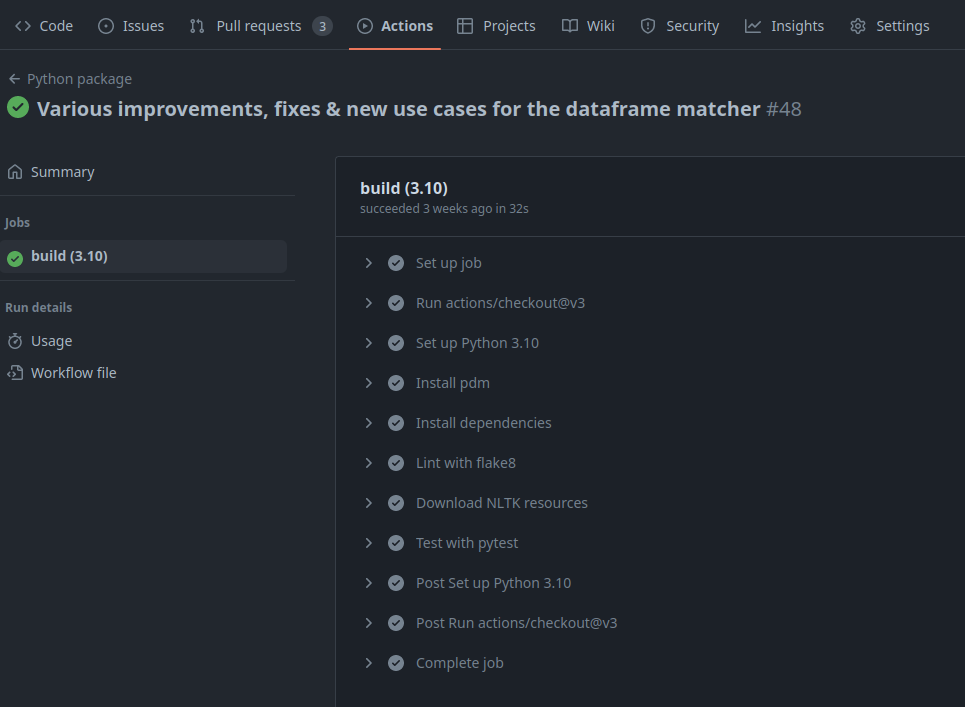
\includegraphics[width=12cm]{figures/discovery_library/test_and_lint_github_action}
    \caption{An example of a single pull request testing and linting action}
    \label{fig:discovery_unit_test}
\end{figure}

We can then further take advantage of these unit tests and the GitHub Actions feature to construct regression tests
that prevent pull requests from accidentally breaking previously working features.
To do this, we configure a GitHub action that runs pytest on our test module, and then require a pull request to have
all tests passing before allowing it to be merged.
In~\ref{fig:discovery_unit_test} we can see an example of the action running in a pull request, additionally we have
used the Flake8~\cite{Flake8} linter to ensure that code conventions have been met.

\subsubsection{Distribution}
With the tool developed, we must find a rational way to distribute the tool to potential users, and how we will provide
them access to documentation of the project functionality.

\begin{figure}[H]
    \centering
    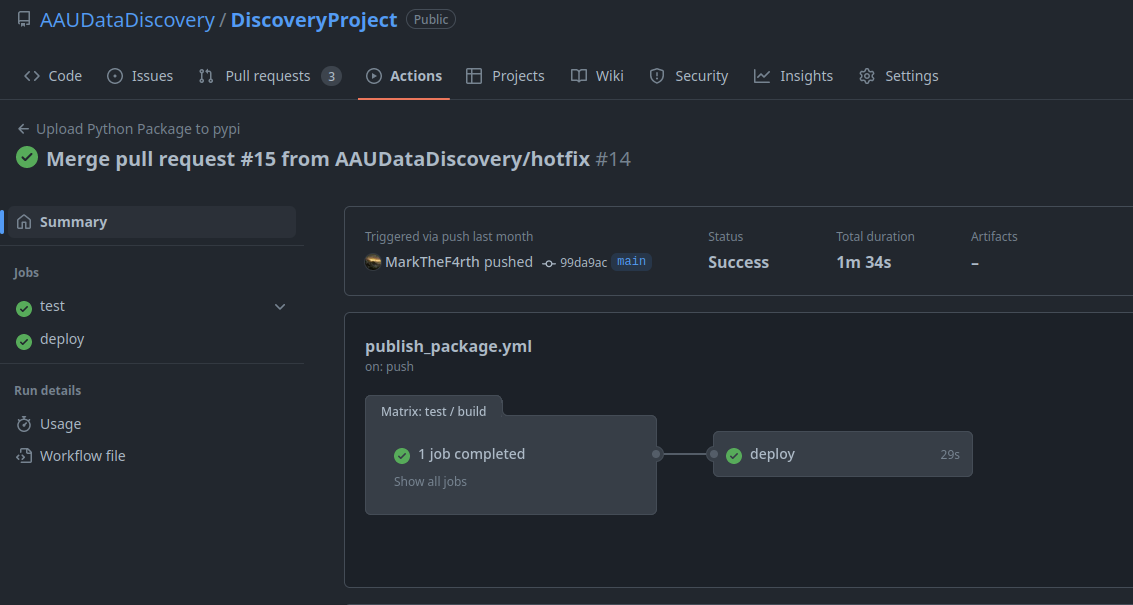
\includegraphics[width=12cm]{figures/discovery_library/github_action_test_and_deploy}
    \caption{An example of a completed pull request, running the test action and then deploying}
    \label{fig:discovery_test_and_deploy}
\end{figure}

\begin{figure}[H]
    \centering
    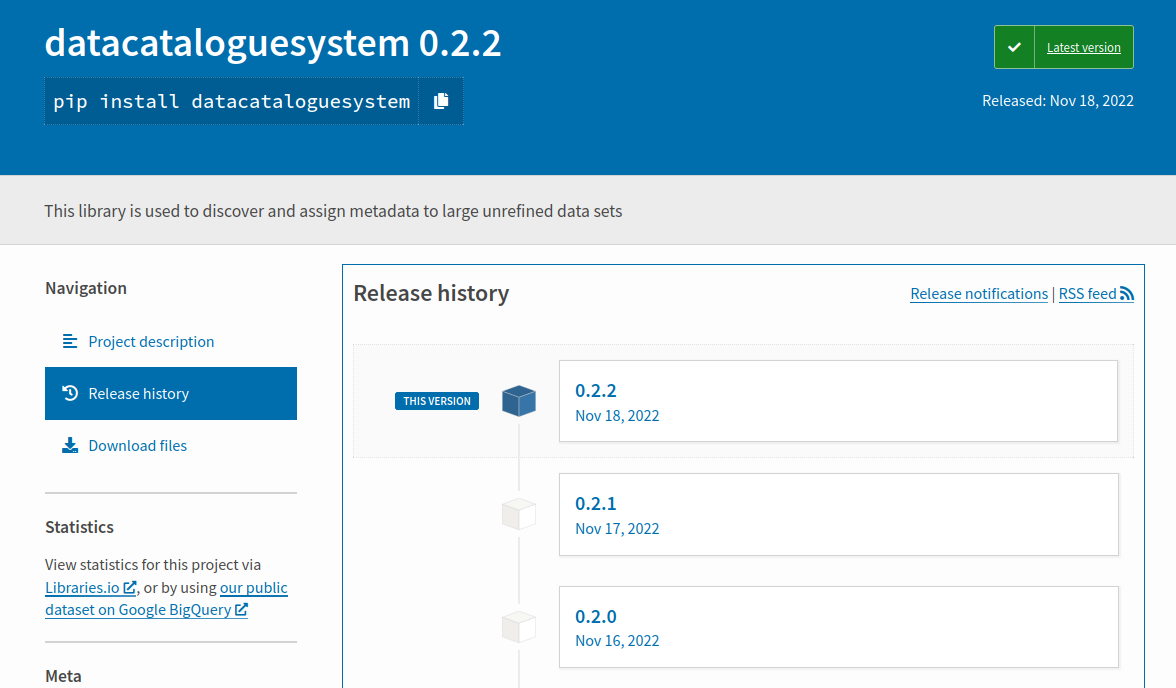
\includegraphics[width=12cm]{figures/discovery_library/pypi_catalogue_upload}
    \caption{The release history of the deployed catalogue system library}
    \label{fig:discovery_pypi_upload}
\end{figure}

Open source python libraries rely on a central public repository called pypi~\cite{PyPi} - to ensure that users have
ease of access to our project, we will similarly host the library there.
With an account created, the only real work involved in this step is to create a pipeline for uploading new releases to
the pypi repository.
For this purpose we can look back to pdm, which has an in-built publishing tool, allowing us to simply create a new
GitHub action responsible for running the \textbf{publish} command which is illustrated
in~\ref{fig:discovery_test_and_deploy}.
With all these steps complete, we can demonstrate the library being accessible on PyPi as in
figure:~\ref{fig:discovery_pypi_upload}.

Lastly, we must document the library, allowing users to have a reference guide for its usage.
For this purpose we will be using the open source documentation tool~\cite{Sphinx}, a tool which features an automatic
documentation library that allows us to build documentation based on python docstrings.
Using the auto documentation feature, we can build a static html file that lists the features of our application,
allowing not only accessible, but easily updatable documentation.
With the documentation html generated, we can use AWS to host a static website that is publicly available.

\begin{figure}[H]
    \centering
    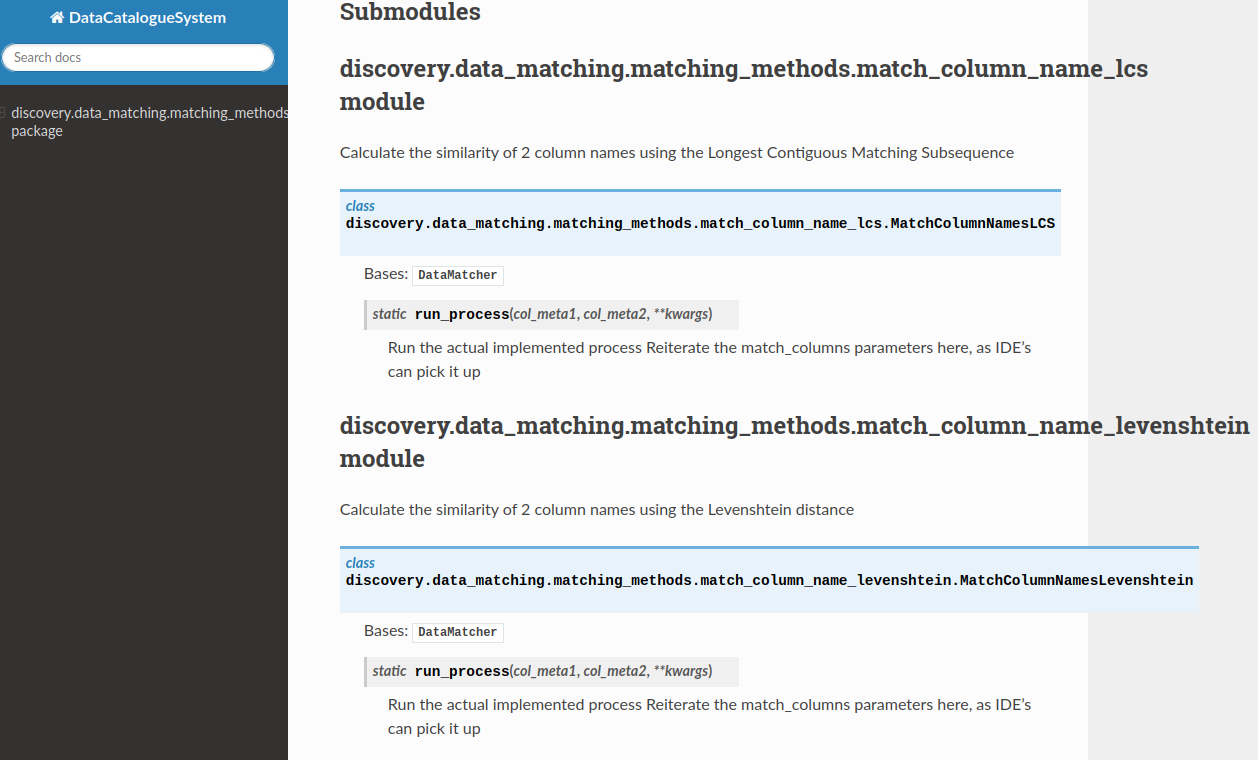
\includegraphics[width=12cm]{figures/discovery_library/discovery_client_documentation}
    \caption{A snippet of the data matching methods within the automatically generated documentation}
    \label{fig:discovery_client_documentation}
\end{figure}

We can see the results of the automatic documentation in~figure~\ref{fig:discovery_client_documentation}, unfortunately
the presentation does require some tweaking before being presentable to end users, however this is a good example of how
easy it is to set up something useful with minimal effort.

\subsubsection{Reflections}
From the beginning, we built the library with future additions in mind, we believe that the structure we built has
managed to adequately achieve a robustness that allows for more specialised features to be created in the future.
Creating new methods for data matching, data loading, or utilities that perform various analytics - all of these can be
easily built on top of the existing structure without significant edits.


\chapter{Conclusion}\label{ch:conclusion}

\section{Answering The Problem Statement}

\section{Future Considerations}

\section{Discussion}
\cite{Madsen2010}
\printbibliography[heading=bibintoc]
\end{document}